\chapter{Experimentos Realizados}
\thispagestyle{plain}
\label{cap:experimentos}
\graphicspath{{./Cap4_Experimentos_Realizados/Figures/}}

A realização dos experimentos baseou-se na utilização da ferramenta de parametrização e obtenção de métricas, aplicado nas imagens tratadas de cada cena, conforme variações definidas no Capítulo anterior. Os dados obtidos foram organizados de forma a facilitar a análise e comparação entre as variações em cada cena e também entre os diferentes dispositivos sendo testados.

Para cada variação de resolução, que depende de uma nova seleção de parâmetros, será exibido a matriz de resultados final juntamente com as faces detectadas, após já feita a análise para se chegar a um melhor resultado, indicando quais foram os parâmetros definidos.

\section{Cena 1}

\subsection{Otimização de parâmetros}

Primeiramente, foi realizada a otimização dos parâmetros para cada variação de resolução, a partir das imagens com todas as faces disponíveis de cada resolução. No caso desta cena, que exige relativamente muito mais processamento, utilizou-se o Raspberry Pi 4B para a definição dos parâmetros, repetindo-os nos testes com o Raspberry Pi Zero W para base de comparação.

A definição dos parâmetros 'ótimos' não é objetiva. Para esta cena, buscou-se um melhor resultado em que houvesse a maior quantidade de faces detectadas com o mínimo ou nenhuma presença de falsos positivos e no menor tempo. Durante a análise, teve-se a razoabilidade de considerar na comparação entre os diferentes resultados da matriz que, um grande aumento no tempo de detecção não justifica um pequeno ganho relativo na quantidade de faces detectadas.

As próximas três subsubseções \ref{sssec:resolution1-1}, \ref{sssec:resolution1-2} e \ref{sssec:resolution1-3} mostram através de imagens, para cada resolução testada, a última iteração da matriz de resultados com os dados entrada, a célula destacada com os parâmetros escolhidos e a imagem com a faces detectadas, nos testes feitos com o Raspberry Pi 4B. 

Os parâmetros definidos de cada resolução foram usados para obter as métricas de cada variação de quantidade de faces detectáveis, e em ambos os dispositivos testados. Não será apresentado nesse documento cada resultado das métricas obtidos em tela. Todos os dados obtidos foram tabelados e utilizados para as comparações feitas nas subseções seguintes. Uma tabela resumida com esses dados é exibida no final de cada uma das próximas três subseções.


\subsubsection{Resolução 1440p} \label{sssec:resolution1-1}

Para essa resolução de 1440 x 2560 conseguiu-se chegar a uma quantidade muito boa de faces detectadas, mesmo as faces menores, de pessoas mais distantes, quase totalizando a quantidade de faces presentes na imagem. Como é normal, algumas faces não foram detectadas devido a algum adereço como chapéu, posição da face e outros possíveis fatores. Nesse caso, nenhum falso positivo foi detectado.

Parâmetros definidos: 
\begin{itemize}
    \SingleSpacing
    \item Min. Size Face: 0.8\%
    \item Scale Factor: 1.069
    \item Min. Neighbors: 3
\end{itemize}

\begin{figure}[H]
    \centering
    \caption[Otimização Cena 1 - resolução 1440p.]{Otimização Cena1 resolução 1440p.}
    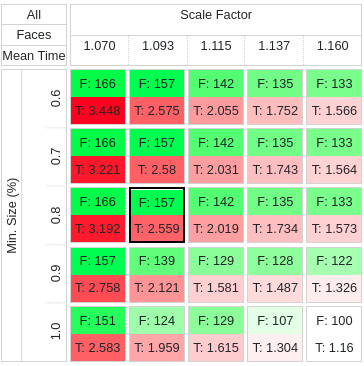
\includegraphics[width=0.70\textwidth]{Cap4_Experimentos_Realizados/Figures/cena1_param_1440p_matriz.jpg}
    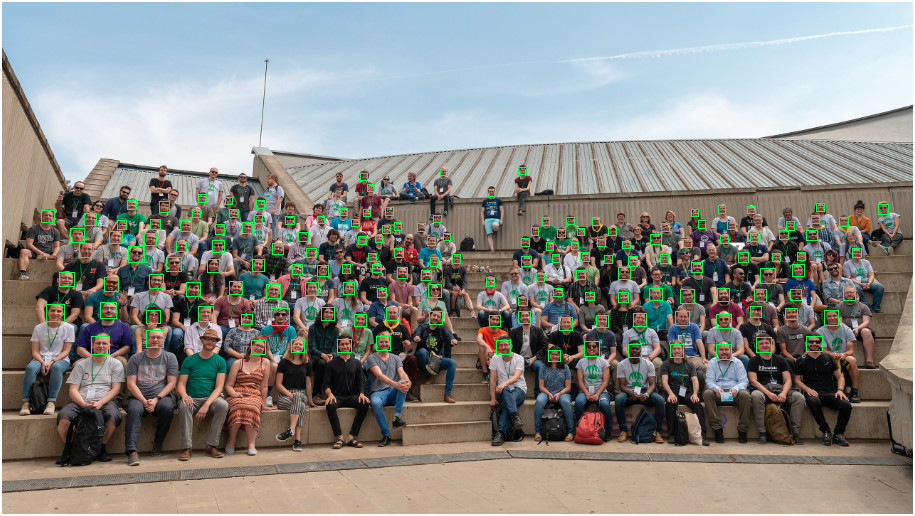
\includegraphics[width=0.85\textwidth]{Cap4_Experimentos_Realizados/Figures/cena1_param_1440p_faces.jpg}
    \caption*{Fonte: compilação do autor.\footnotemark}
    \label{fig:otimizacaoCena1_1440p}
\end{figure}

\footnotetext{Imagem usada na compilação disponível em: <https://commons.wikimedia.org/wiki/File:Wikimedia\_Hackathon\_Barcelona\_2018\_-\_group\_photo.jpg>
Arquivo de imagem sob a licença CC BY-SA 4.0: <https://creativecommons.org/licenses/by-sa/4.0/deed.en>}
    
\begin{table}
    \centering
    \caption[Dados obtidos - resolução 1440p.]{Dados obtidos - resolução 1440p.}
    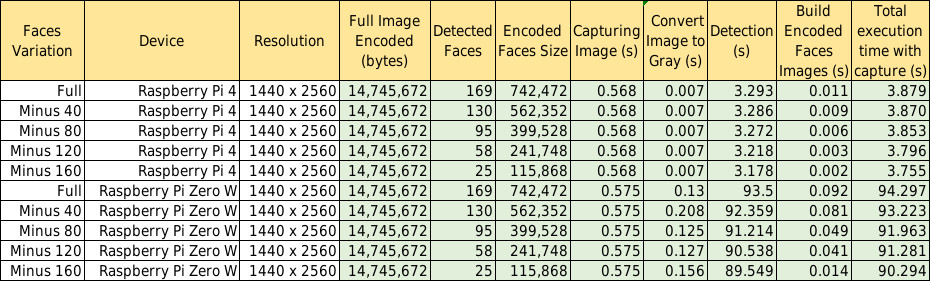
\includegraphics[width=0.90\textwidth]{Cap4_Experimentos_Realizados/Figures/cena1_dados_1440p.jpg}
    \caption*{Fonte: autor.}
    \label{fig:dadosCena1_1440p}
\end{table}

\subsubsection{Resolução 1080p} \label{sssec:resolution1-2}

Nessa resolução de 1080 x 1920, algumas faces menores começam a não serem mais detectadas, mas a quantidade de faces detectadas é relativamente grande se comparado à quantidade de faces presentes na imagem.

Observa-se uma diminuição no valor do parâmetro scale factor (que significa mais passos no escalonamento da imagem) para se obter quantidades maiores de faces detectadas e um aumento no do parâmetro min. size, já que as faces menores começam a ficar indetectáveis.

Dessa vez percebe-se a presença de alguns falsos positivos. Testou-se a variação do parâmetro min. neighbors, porém não houve melhoria.

Parâmetros definidos: 
\begin{itemize}
    \SingleSpacing
    \item Min. Size Face: 1.0\%
    \item Scale Factor: 1.039
    \item Min. Neighbors: 3
\end{itemize}

\begin{figure}[H]
    \centering
    \caption[Otimização Cena 1 - resolução 1080p.]{Otimização Cena1 resolução 1080p.}
    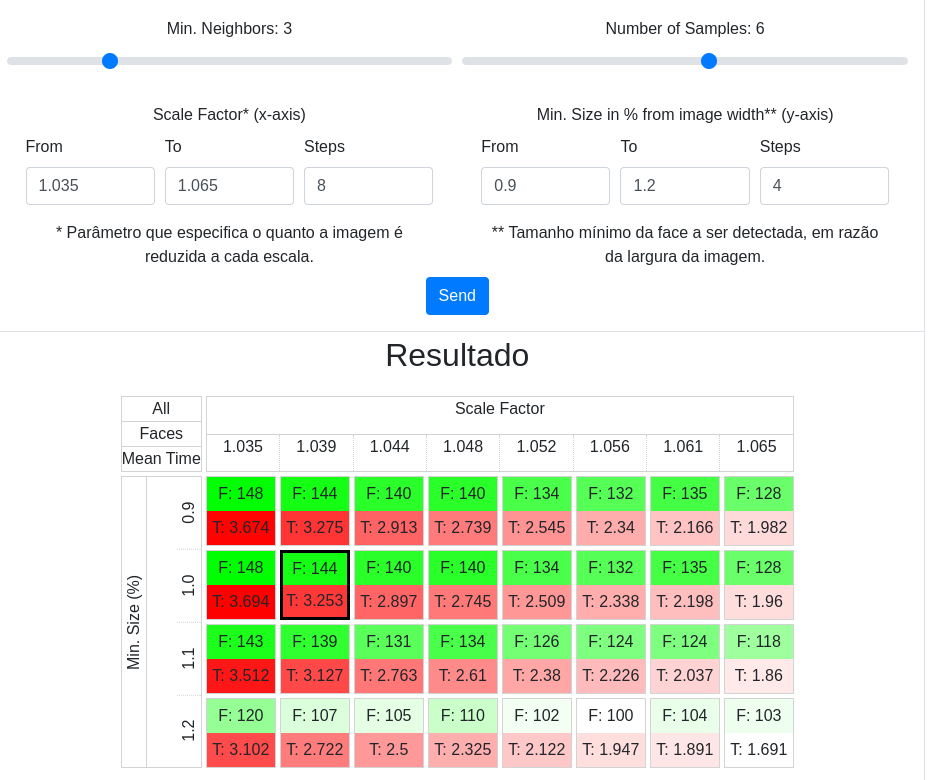
\includegraphics[width=0.70\textwidth]{Cap4_Experimentos_Realizados/Figures/cena1_param_1080p_matriz.jpg}
    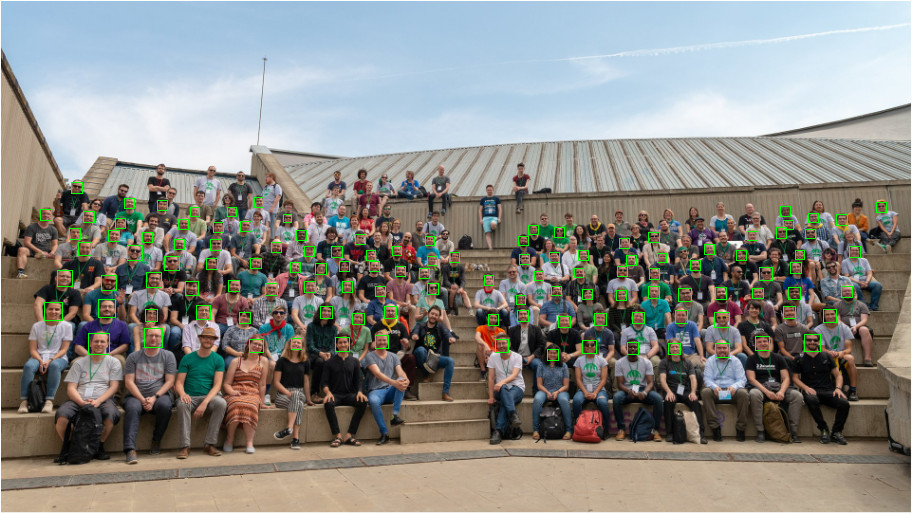
\includegraphics[width=0.85\textwidth]{Cap4_Experimentos_Realizados/Figures/cena1_param_1080p_faces.jpg}
    \caption*{Fonte: compilação do autor.\footnotemark[\value{footnote}]}
    \label{fig:otimizacaoCena1_1080p}
\end{figure}

\begin{table}
    \centering
    \caption[Dados obtidos - resolução 1080p.]{Dados obtidos - resolução 1080p.}
    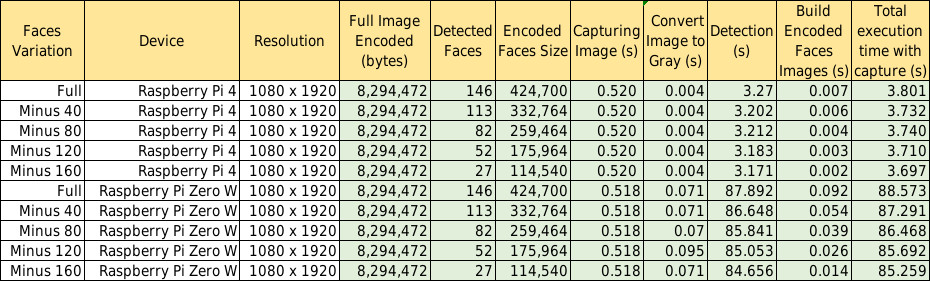
\includegraphics[width=0.90\textwidth]{Cap4_Experimentos_Realizados/Figures/cena1_dados_1080p.jpg}
    \caption*{Fonte: autor.}
    \label{fig:dadosCena1_1080p}
\end{table}

\subsubsection{Resolução 720p} \label{sssec:resolution1-3}

Nessa resolução de 720 x 1280, a queda na quantidade de faces detectadas já se torna bem considerável se comparando às resoluções maiores, sendo menos de um terço da quantidade de faces presente na imagem. Novamente, observa-se a diminuição do parâmetro de scale factor e aumento do parâmetro min. size, devido às faces menores não detectáveis.
Também percebe-se a presença de falso positivo. Testou-se também a variação do parâmetro min. neighbors. Aumentando-se de 3 para 4, observou-se a redução de falsos positivos.

Parâmetros definidos: 
\begin{itemize}
    \SingleSpacing
    \item Min. Size Face: 1.6\%
    \item Scale Factor: 1.024
    \item Min. Neighbors: 4
\end{itemize}

\begin{figure}[H]
    \centering
    \caption[Otimização Cena 1 - resolução 720p.]{Otimização Cena 1 - resolução 720p.}
    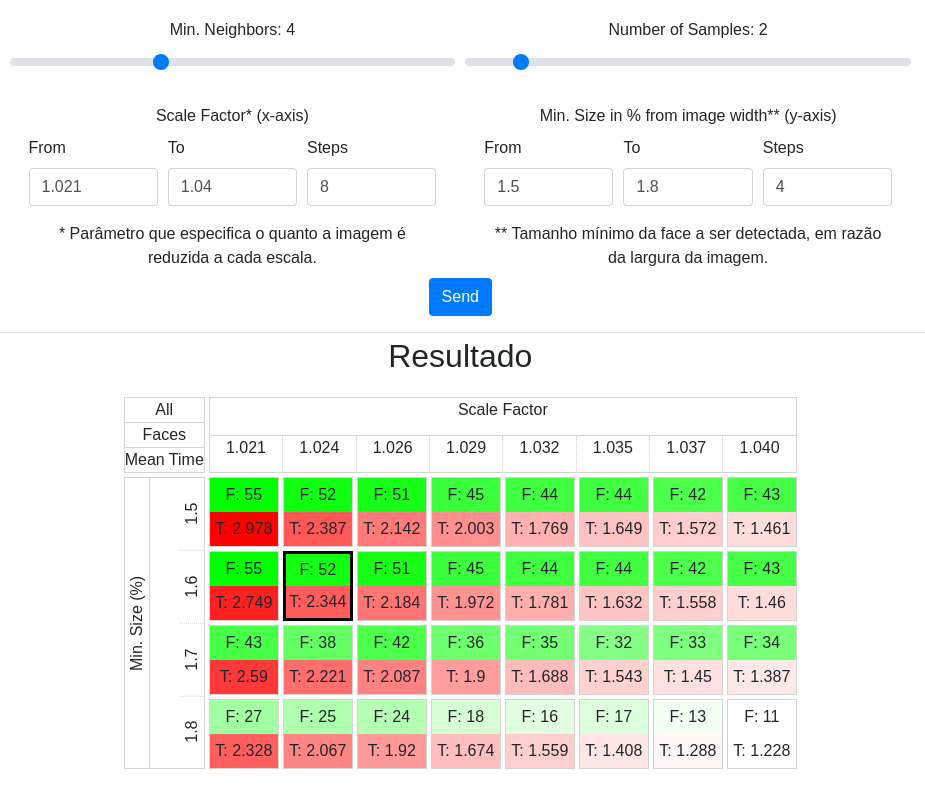
\includegraphics[width=0.70\textwidth]{Cap4_Experimentos_Realizados/Figures/cena1_param_720p_matriz.jpg}
    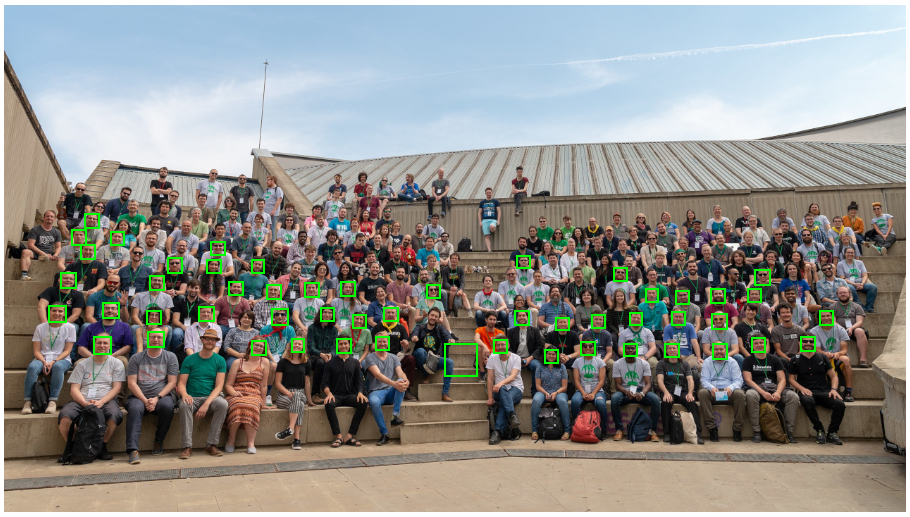
\includegraphics[width=0.85\textwidth]{Cap4_Experimentos_Realizados/Figures/cena1_param_720p_faces.jpg}
    \caption*{Fonte: compilação do autor.\footnotemark[\value{footnote}]}
    \label{fig:otimizacaoCena1_720p}
\end{figure}

\begin{figure}
    \centering
    \caption[Tabela de Dados - resolução 720p.]{Tabela de Dados - resolução 720p.}
    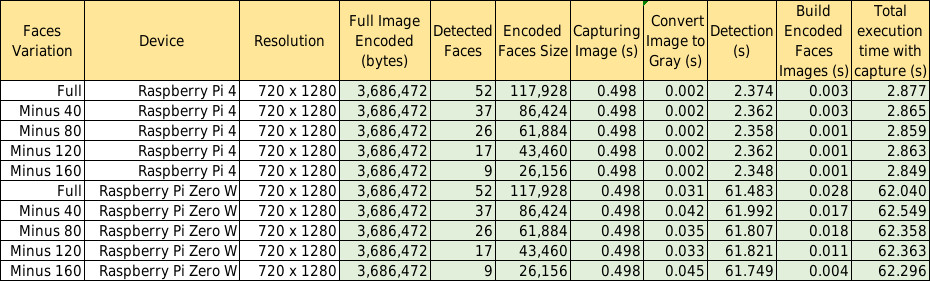
\includegraphics[width=0.90\textwidth]{Cap4_Experimentos_Realizados/Figures/cena1_dados_720p.jpg}
    \caption*{Fonte: autor.}
    \label{fig:dadosCena1_720p}
\end{figure}

\subsection{Análise dos resultados}
Nesta cena, são três fatores influenciando no resultado das detecções, seja quanto à capacidade de detecção e/ou quanto ao tempo de resposta. Esses fatores são a quantidade de faces detectáveis presentes na imagem, a resolução da imagem e o dispositivo rodando o algoritmo de detecção, sobre os quais serão feitas as comparações e análises a seguir.

\subsubsection{Efeitos da variação por quantidade de faces}

Os gráficos apresentados na figura \ref{fig:dadosCena1_graficos_variacao_faces} foram montados de forma a facilitar o entendimento de como a quantidade de faces influencia no tempo de detecção. Para maior clareza, os dados foram apresentados em três gráficos diferentes, um para cada resolução de imagem.
No eixo x, têm-se as variações de quantidade de faces detectáveis disponíveis. "Full" \ refere-se à imagem original, sem alteração, com todas as faces detectáveis, "Minus 40" \ refere-se à imagem trabalhada para borrar 40 faces de forma distribuída, tornando-as indetectáveis, e assim por diante.

Há três séries de dados cujas métricas são apresentadas para cada variação de faces. A quantidade de faces detectadas pelo algoritmo representada pelas barras verdes, que seguem a escala do eixo y à esquerda; o tempo total de execução nos testes com o Raspberry Pi 4B. em azul escuro, e o tempo total de execução nos teste com o Raspberry Pi Zero, em azul claro, ambos sguindo a escala do eixo y à direita, com unidade em segundos. Para melhor visualização, o eixo y à direita está em escala logarítmica.
O tempo de execução total é a soma do tempo de aquisição de imagem (nesse caso já considerando o tempo de captura do módulo câmera e não de leitura da imagem em arquivo), o tempo de conversão da imagem em escala de cinza, o tempo de detecção em si e o tempo de encodamento da imagem para transporte.
Há também a representação no gráfico, em linha amarela tracejada, do tempo de 5 segundos definido como limite para atender ao requisito da cena.

A ferramenta utilizada para a geração dos gráficos a partir da tabela de dados foi o \emph{Data Studio} \cite{DataStudio}, da Google.

Como se pode notar pela análise dos gráficos, a variação da quantidade de faces presentes, e por consequência detectadas, influencia muito pouco no tempo de detecção, chegando a 4\% a maior diferença. Observa-se esse comportamento em ambos os dispositivos testados e em todas a resoluções de imagem.

Com base nisso, pode-se dizer que, para a cena em questão, a quantidade de pessoas presentes no ambiente pouco no tempo de resposta do algoritmo em uso, o \textit{Haar cascade object detection} \cite{Viola2001}, podendo então este fator ser desconsiderado para quesitos de tempo (mas não de utilização de banda, obviamente).

\begin{figure}[H]
    \centering
    \caption[Faces detectadas e Tempos de execução por Variação de faces detectáveis.]{Faces detectadas e Tempos de execução por Variação de faces detectáveis.}
    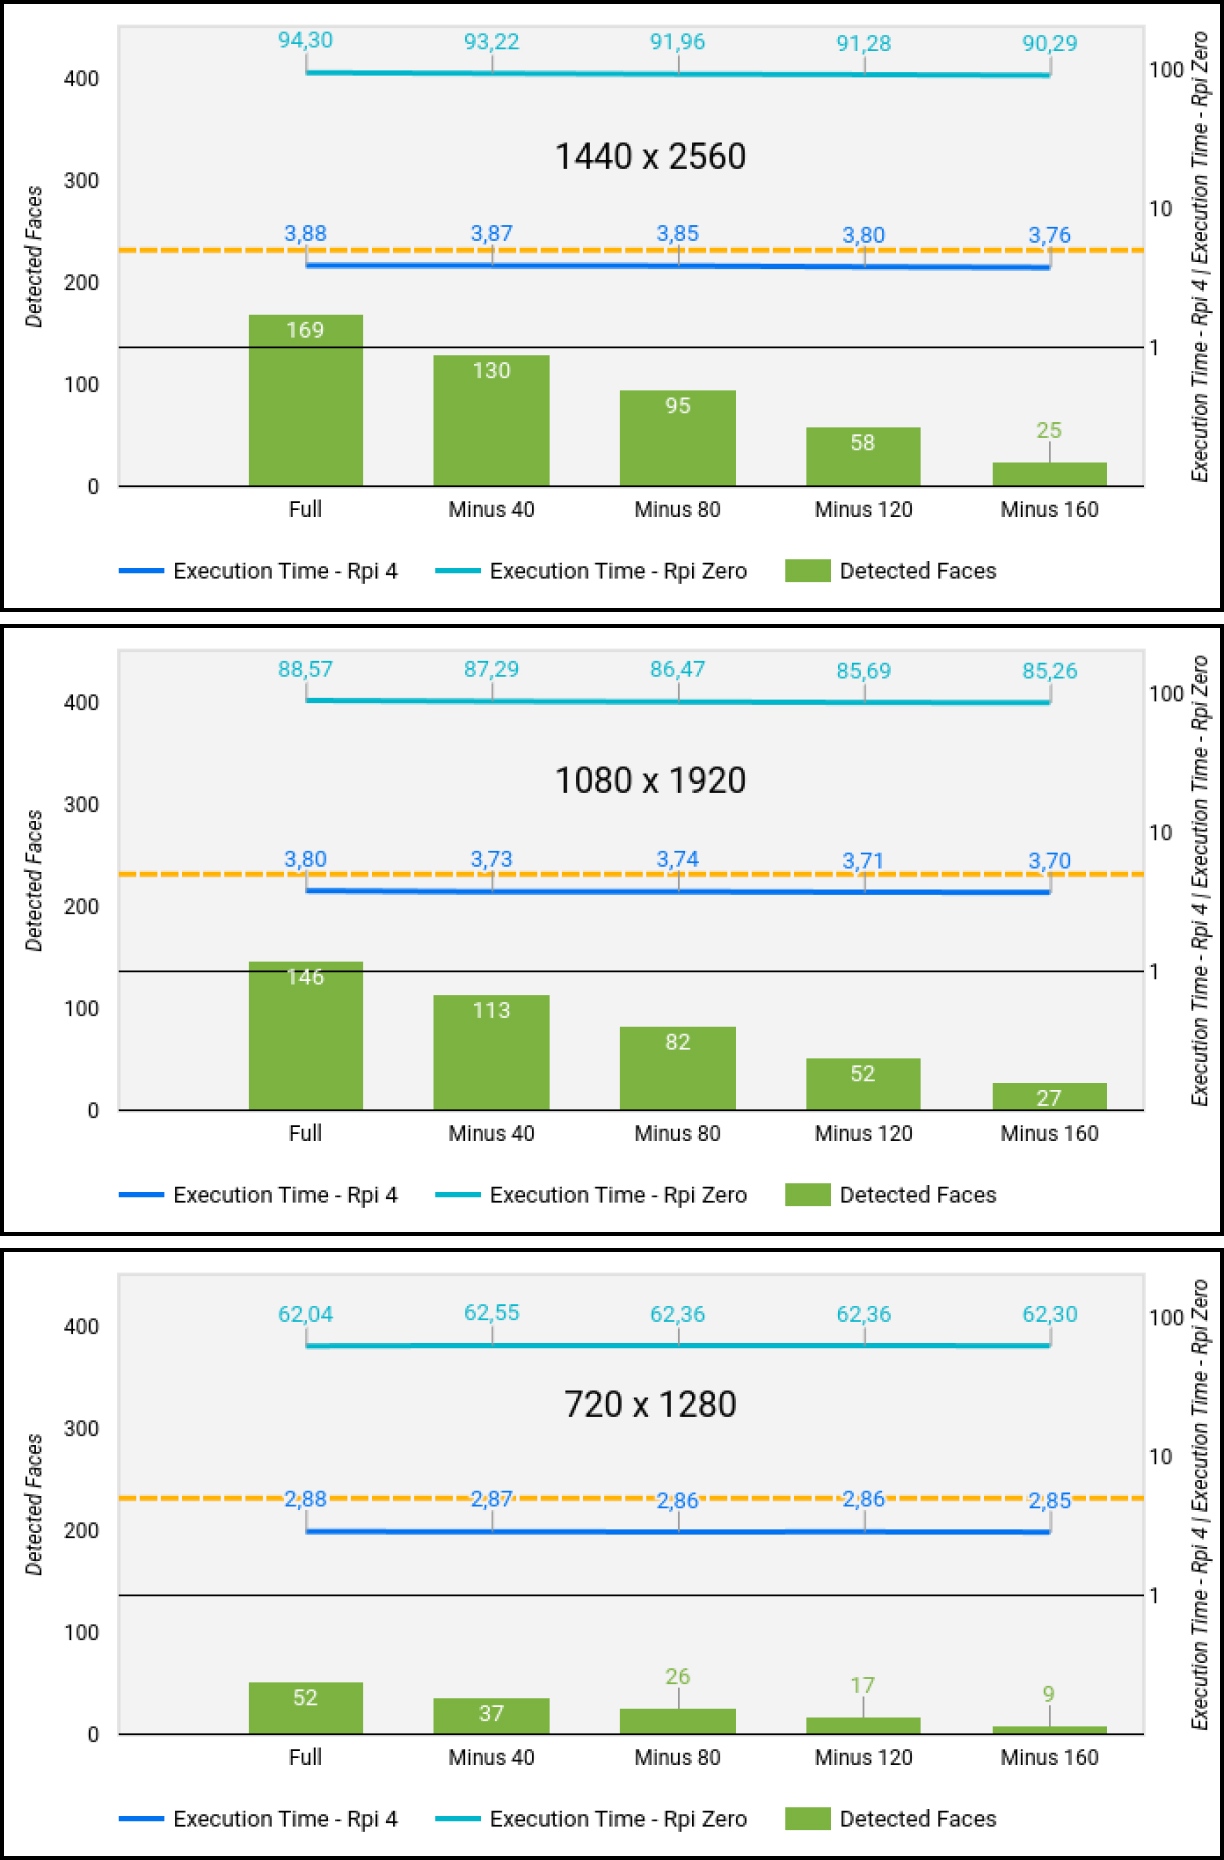
\includegraphics[width=0.7\textwidth]{Cap4_Experimentos_Realizados/Figures/cena1_graficos_variacao_faces.jpg}
    \caption*{Fonte: autor.}
    \label{fig:dadosCena1_graficos_variacao_faces}
\end{figure}

\subsubsection{Efeitos da variação por resolução de imagem}

Como foi constatado que a variação da quantidade de faces tem efeito insignificante no tempo de resposta, considerou-se apenas os resultados dos testes nas imagens com todas as faces detectáveis para montar o gráfico da figura \ref{fig:cena1_graficos_variacao_resolucao}, que têm a mesma estrutura dos gráficos anteriores, com a exceção de que no eixo x têm agora a variação por resolução de imagem.

Ao se comparar as duas maiores resoluções, 1440p e 1080p, observa-se que tanto o tempo de execução quanto o a quantidade de faces detectadas são menores na resolução menor, como é de se esperar. A redução no tempo é muito pouco expressiva, enquanto a redução na quantidade de faces detectadas não é tão expressiva mas pode-se considerar razoável.
Comparando-se as faces detectadas nessa duas resoluções, vide figuras \ref{fig:otimizacaoCena1_1440p} e \ref{fig:otimizacaoCena1_1080p}, percebe-se que as faces não detectadas são de pessoas que estão mais distantes na cena. Essa diferença de 25 faces (desconsiderando-se 2 falsos positivos na resolução de 1080p) pode ou não fazer grande diferença para a tomada de decisão, vai depender da realidade da cena real, se seria comum pessoas posicionadas tão distantes sem se aproximar da câmera, etc. 

É de se pensar que tendo menor resolução, a redução no tempo de resposta deveria ser razoavelmente menor devido à quantidade menor de pixels e quadros sendo processados. Porém, deve-se considerar também que, ao se buscar a maximização da quantidade de faces detectadas, reduziu-se o valor do parâmetro \emph{scale factor} durante a otimização, o que aumenta a quantidade de iterações no escalonamento. Comparando-se as matrizes de resultado nas figuras \ref{fig:otimizacaoCena1_1440p} e \ref{fig:otimizacaoCena1_1080p}, à medida que se caminha para a direita na matriz refente à resolução de 1080p, com valores maiores de \emph{scale factor} se aproximando ao selecionado para 1440p, observa-se uma redução considerável no tempo de detecção, com esperado, porém com também considerável redução na quantidade de faces detectadas.

Já comparando-se os resultados obtidos com a imagem de menor resolução, 720p, e as demais, a perda com relação à quantidade de faces detectadas é bastante expressiva, chegando a cair para menos de um terço da quantidade de faces detectadas na imagem de 1440p. Como pode ser visto na imagem \ref{fig:otimizacaoCena1_720p}, apenas as faces maiores (de pessoas mais próximas da câmera) são detectadas. A tempo de resposta tem uma queda até que razoável, porém não compensa a perda na quantidade de faces detectadas. Dessa forma, o uso de imagens com resolução de 720p se torna inadequado para o cenário em questão. 

\begin{figure}[h]
    \centering
    \caption[Faces detectadas e Tempos de execução por Variação de resolução.]{Faces detectadas e Tempos de execução por Variação de resolução.}
    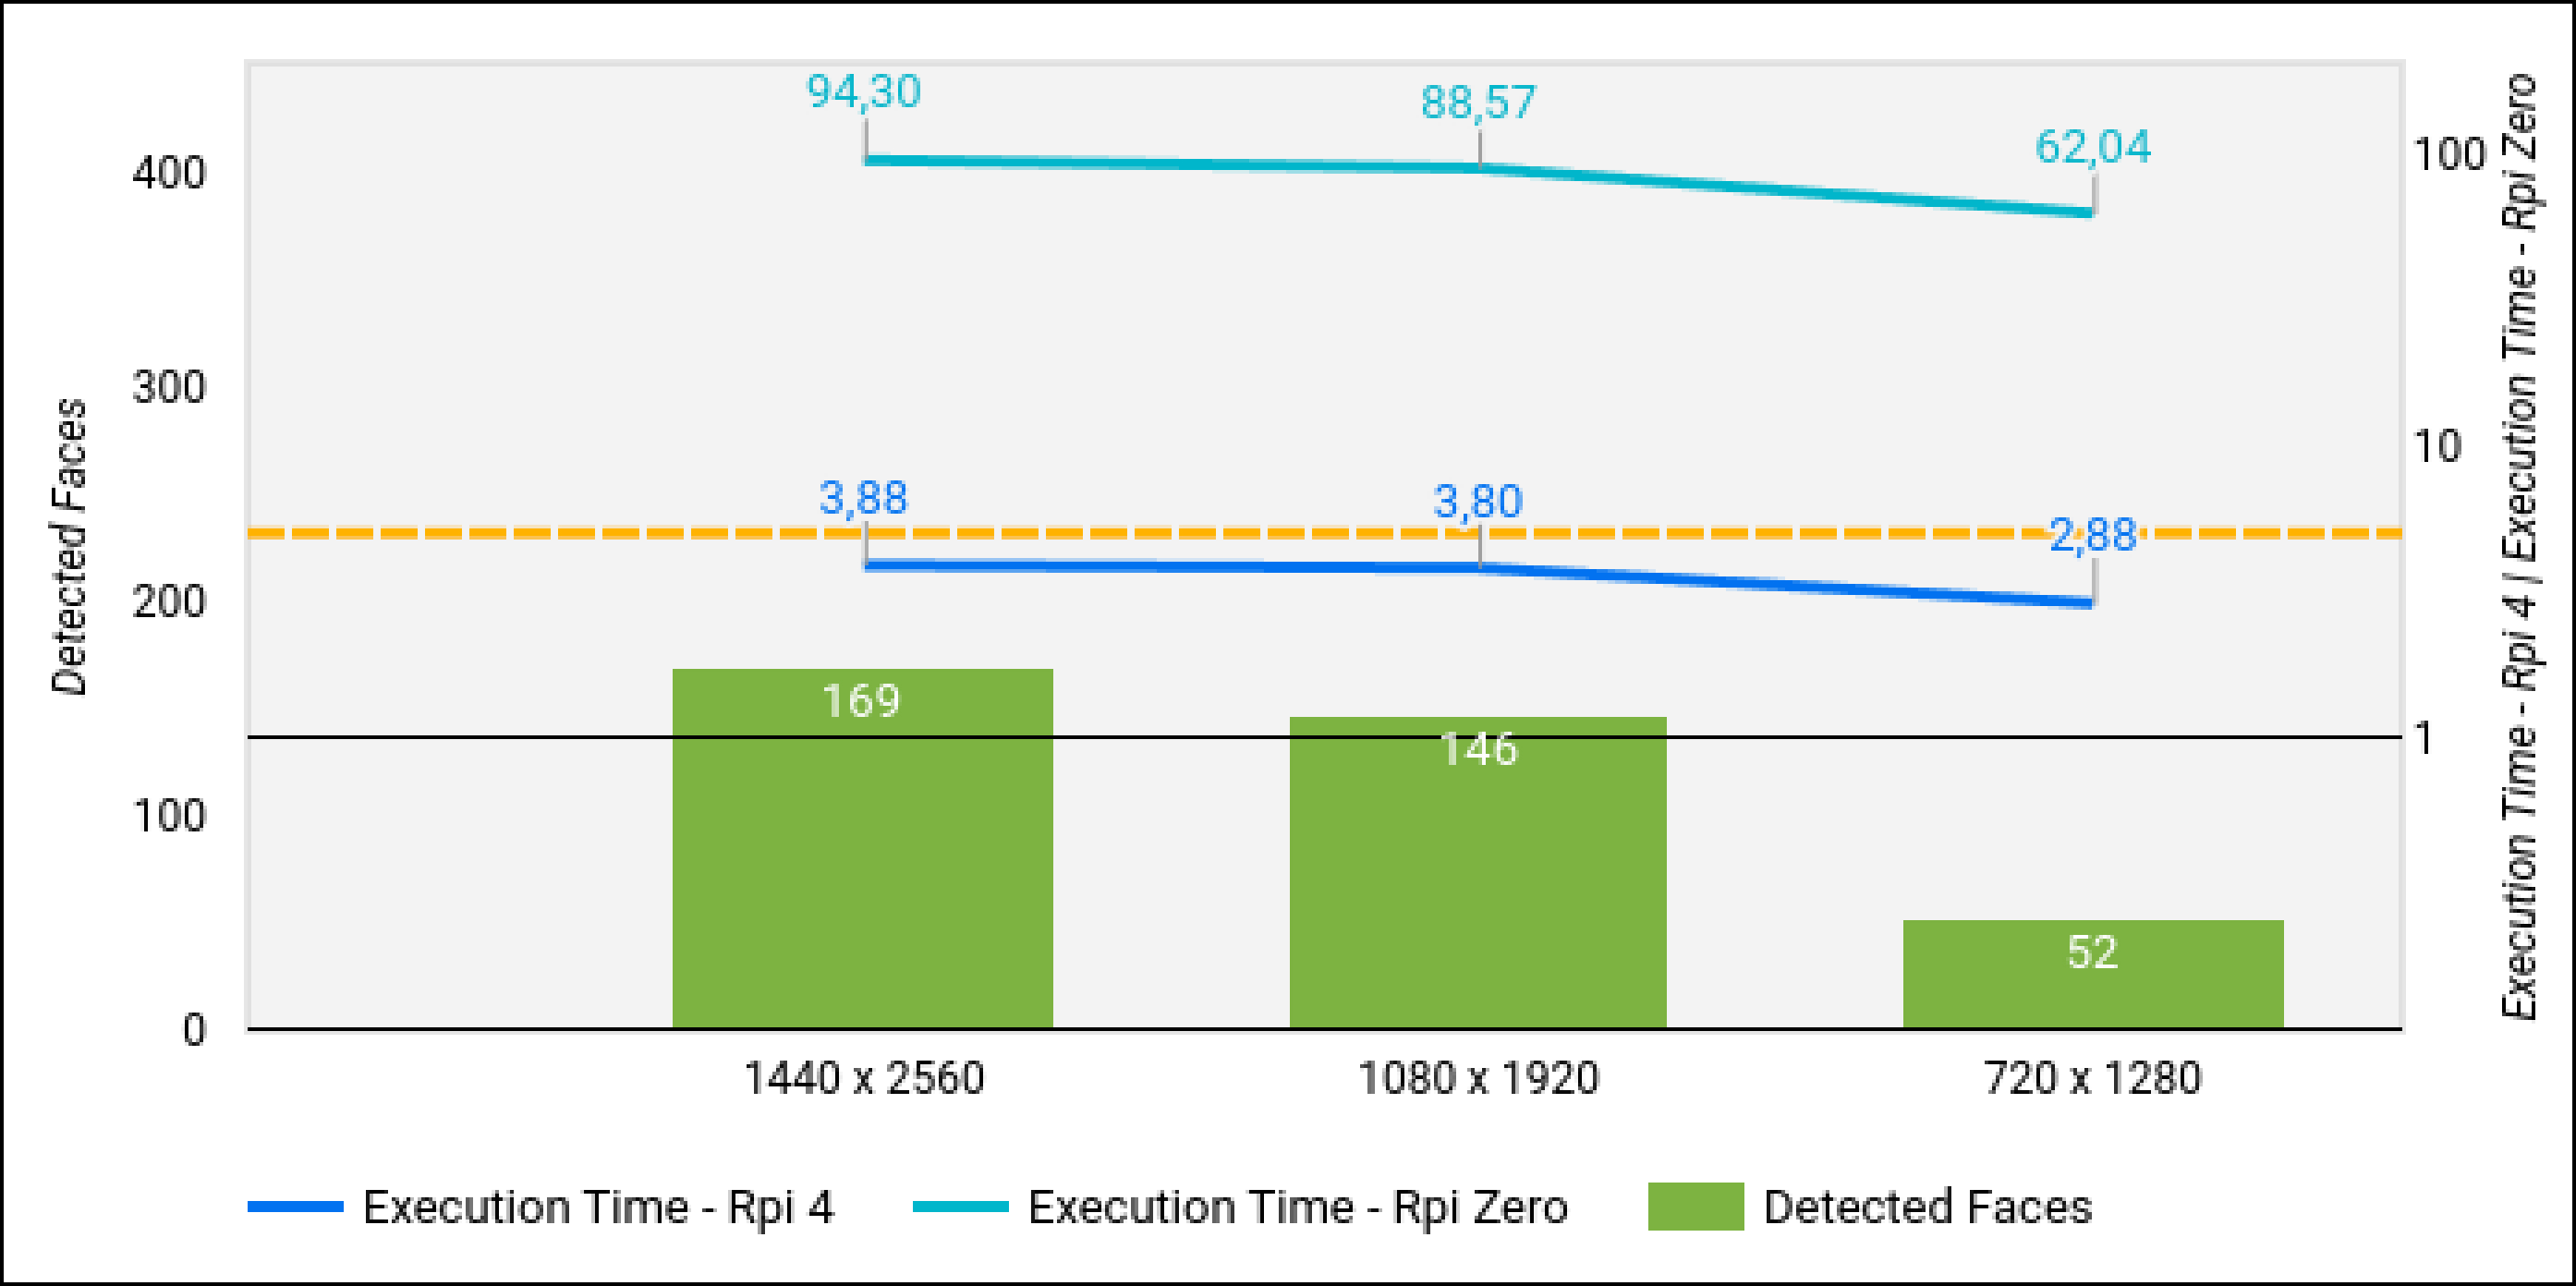
\includegraphics[width=0.7\textwidth]{Cap4_Experimentos_Realizados/Figures/cena1_graficos_variacao_resolucao.jpg}
    \caption*{Fonte: autor.}
    \label{fig:cena1_graficos_variacao_resolucao}
\end{figure}

Pode-se afirmar então que, a princípio, considerando-se apenas o \emph{trade-offf} entre quantidade de faces detectadas e tempo de resposta, a resolução de 1440p, a maior entre as  testadas, se mostra a mais adequada a se utilizar nesse tipo de cenário, onde objetiva-se detectar o máximo de faces possível e de tamanhos relativos muito pequenos.

Outra questão em que a utilização de resolução maior torna-se vantajoso é quanto à qualidade das imagens recortadas das faces. Caso as imagens das faces sejam utilizadas em uma próxima etapa da aplicação em outro dispositivo na rede ou na nuvem, como por exemplo para reconhecimento facial ou simplesmente manter em registro, a qualidade e detalhes da face recortada pode fazer diferença no sucesso dessa próxima etapa.

Para se ter uma ideia mais visual da diferença, a figura \ref{fig:cena1_comparativo_qualidade_faces} faz um comparativo entre duas faces detectadas (a de uma pessoa mais próxima e a de uma pessoa mais distante) e as diferentes resoluções.

\begin{figure}[h]
    \centering
    \caption[Comparativo de faces recortadas de diferentes resoluções, em tamanho real.]{Comparativo de faces recortadas de diferentes resoluções, em tamanho real.}
    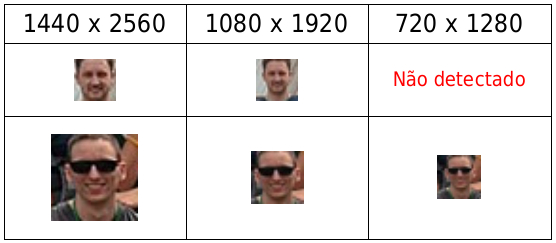
\includegraphics[width=0.8\textwidth]{Cap4_Experimentos_Realizados/Figures/cena1_comparativo_qualidade_faces_recortadas.jpg}
    \caption*{Fonte: autor.}
    \label{fig:cena1_comparativo_qualidade_faces}
\end{figure}

Um fator que talvez possa pesar a favor de se utilizar resolução menor é a quantidade de dados sendo trafegados ou armazenados. A figura \ref{fig:cena1_comparativo_tamanho_faces} traz um comparativo entre o tamanho médio das imagens das faces recortadas, coloridas e encodadas em base64. Nesse caso, observa-se que a utilização da resolução em 1080p reduziria o tamanho de dados trafegados e/ou armazenados em aproximadamente 34\%. Claro que existe a possibilidade de realizar a detecção na resolução maior e redimensionar as imagens antes de serem transmitidas, mas deve-se levar em consideração que, para tal, haverá mais carga de processamento no dispositivo de borda.

\begin{figure}[h]
    \centering
    \caption[Comparativo de tamanho médio de imagem encodada por face detectada em bytes.]{Comparativo de tamanho médio de imagem encodada por face detectada em bytes.}
    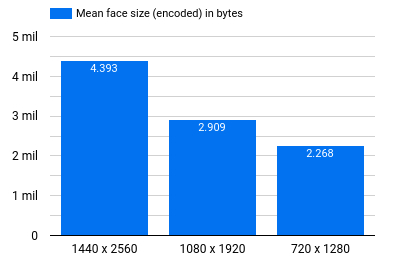
\includegraphics[width=0.65\textwidth]{Cap4_Experimentos_Realizados/Figures/cena1_graficos_tamanho_medio_imagem_face.jpg}
    \caption*{Fonte: autor.}
    \label{fig:cena1_comparativo_tamanho_faces}
\end{figure}

\subsubsection{Considerações sobre os dispositivos testados}
Nos gráficos apresentados nas figuras \ref{fig:dadosCena1_graficos_variacao_faces} e \ref{fig:cena1_graficos_variacao_resolucao} já fica bem evidente que o Raspberry Pi Zero W deixa a desejar, com tempos de resposta acima de 1 minuto, muito além do aceitável para a cena. Pode-se concluir então que a utilização deste não é adequada para processamento de detecção de faces em imagens com resoluções mais altas, como as testadas, independete da quantidade de faces presentes na imagem.

Já o Raspberry Pi 4B apresentou bom desempenho, conseguindo detectar 169 faces na maior resolução com tempo médio de resposta de 3,88, desde a captura do frame até a preparação das faces cortadas em dados prontos para transmissão. Um tempo razoavelmente menor que o máximo desejado no cenário, com uma margem 22\% e que ainda pode ser aumentada tirando proveito de processamento assíncrono, principalmente na captura dos frames, o que não foi feito nesses testes.

\subsubsection{Considerações sobre utilização de banda}

Quando em uma aplicação com arquitetura distribuída, uma das principais vantagens de se alocar parte do processamento nos dispositivos de borda é a economia que se pode ter na utilização de banda ao trafegar os dados gerados por esses dispositivos para outros positivos que estejam na mesma rede ou na nuvem, que desempenham outras funções dentro da aplicação. Quando se tem têm imagens sendo trafegadas, como é o caso desse estudo, o volume de dados é razoavelmente alto, podendo essa economia ser muito relevante para o projeto.

Trazendo para a cena em questão, caso o dispositivo de borda tivesse a função de apenas capturar a imagem, encodar e transmiti-la para um outro dispositivo realizar a detecação das faces, as imagens teriam que ser transmitidas em sua totalidade para se obter o mesmo resultado. Uma grande quantidade de dados trafegados, refentes às partes das imagens não úteis após a detecção, seriam descartados, desperdiçando-se assim a utilização de banda da rede. Inclusive, mesmo não havendo faces presentes, as imagens precisariam continuar sendo enviadas periodicamente, evidenciando ainda mais o desperdício. Isso pode gerar vários problemas como gargalos na rede e sobrecarga computacional.

Tendo-se a detecção das faces realizada pelo próprio dispositivo na borda, apenas as partes úteis da imagens, que são as faces recortadas, precisam ser transmitidas, proporcionando assim uma utilização mais eficiente na utilização da rede que interliga os diferentes dispositivos.

Durante os testes, junto com as métricas de tempo de processamento são obtidas também as informações do tamanho total da imagem testada e também a soma das imagens das faces recortadas, que serão usadas para comparações na sequência. Estão sendo considerados os tamanhos das imagens após encodamento em base64.

A figura \ref{fig:cena1_comparativo_utilizacao_banda} mostra um comparativo de como seria a utilização de banda nos dois casos, transmitindo-se a imagem completa e transmitindo-se apenas as imagens das faces recortadas, com resolução de 1440 x 2560. Para o cálculo de utilização de banda, considerou-se intervalo entre as detecções de 5 segundos, conforme tempo máximo definido como requisito para esta cena.

No eixo x têm-se a quantidade de faces que foram detectadas, nas barras de cor vermelha a largura de banda que seria utilizada trafegando-se a imagem completa e nas barras de cor verde a largura de banda considerando-se o tráfego apenas do recorte das faces detectadas, ambas seguindo a escala à esquerda do eixo y e expressas em MBps. Na série em formato de linha azul têm-se a diferença percentual em relação ao tamanho da imagem completa, seguindo a escala à direita do eixo y.

\begin{figure}
    \centering
    \caption[Comparativo de utilização de banda por quantidade de faces detectadas.]{Comparativo de utilização de banda por quantidade de faces detectadas.}
    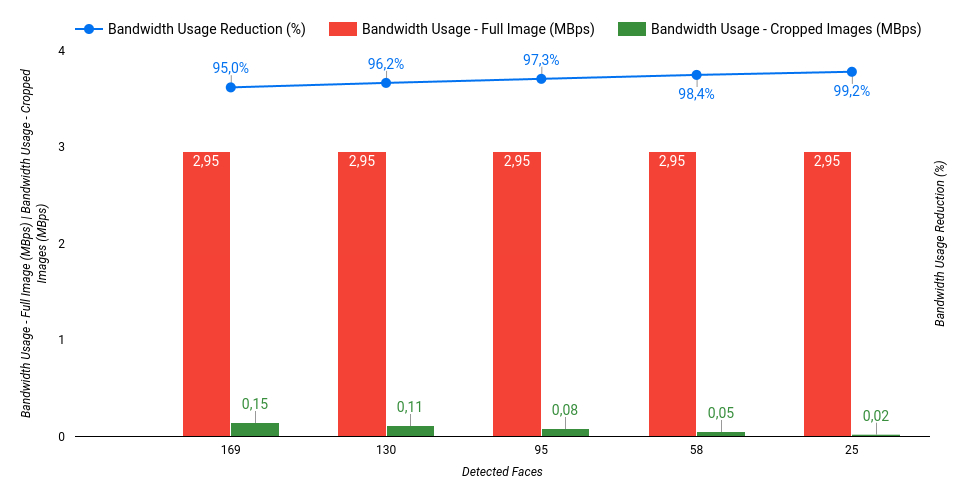
\includegraphics[width=0.95\textwidth]{Cap4_Experimentos_Realizados/Figures/cena1_comparativo_utilizacao_banda.jpg}
    \caption*{Fonte: autor.}
    \label{fig:cena1_comparativo_utilizacao_banda}
\end{figure}

Como se pode observar, a redução na utilização de banda para tráfego das imagens ao se utilizar o processamento na borda para detecção de face é bastante expressivo, partindo-se de 95\% para o caso em que há grande quantidade de faces detectadas (196) e chegando a 99,2\% no caso com muito poucas faces detectadas (25). De fato, a redução pode chegar até a 100\% em eventuais momentos em que não haja face alguma a ser detectada.

Pode-se pensar que talvez a utilização de quase 3 MBps para se transmittir a imagem completa não seria algo tão absurso assim, dependendo da infraestrutura de rede disponível e seu estado de utilização. Mas é importante atentar-se aqui que a unidade sendo usada está em Megabytes/s, então 3 MBps corresponderia a 24 Mbps (Megabits/s), nada mais sendo do que 24\% da capacidade de banda de uma rede operando a 100 Mbps.

Além disso, está se considerando aqui a utilização de banda de apenas um dispositivo. Em uma aplicação real, é razoável considerar que podem haver dezenas de dispositivos realizando monitoramento e tendo de enviar imagens e dados a algum outro dispositivo centralizador, seja em uma rede logal ou algum servidor na nuvem. Imagine um caso com apenas 5 dispositivos de borda distribuídos em ambientes parecidos com a cena em questão, capturando imagens em 1440 x 2560 e a cada 5s para monitoramento e detecção de faces. Caso não haja detecção de face na borda, a utilização de banda necessária para transmissão das imagens completas seria de pelo menos 120 Mbps, o que já seria inviável em uma rede local de 100 Mbps, quanto mais na nuvem.
Agora, considere que todos esses 5 dispositivos tenham capacidade de realizar a detecção transmitir apenas as imagens das faces recortadas. Para o pior caso que se testou, 169 faces detectadas, a banda demandada pelos cinco dispositivos simultaneamente seria de aproximadamente 0,75 MBps, ou 6 Mbps, algo bastante razoável para se trafegar em uma rede local mas talvez ainda nem tanto para se transmitir continuamente pela nuvem.

\section{Cena 2}

\subsection{Captura de imagens para teste}

Conforme definido no capítulo anterior, as imagens para teste foram capturadas a partir de um módulo de câmera conectado no Raspbery Pi 4B.

A cena foi montada conforme pode ser visualizado na figura \ref{fig:cena2_posicao1_visao_externa}. O Raspberry Pi 4B, montado em sua case e com o módulo da câmera conectado foi fixado no batente lateral esquerdo da porta da entrada, de forma que a câmera ficasse posicionada a 1,7m do piso e levemente inclinada para baixo e para a dentro, na direção da passagem. A pessoa que aparece na imagem é o próprio autor.

Utilizando-se o script de captura de frames, foram feitos alguns testes e definiu-se essa como a posição mais próxima para se obter a primeira imagem a ser utilizada nos testes de desempenho, pois consegue pegar uma boa imagem do rosto e ainda com um pouco de folga vertical, considerando-se pessoas mais altas ou baixas.

\begin{figure}[H]
    \centering
    \caption[Posicionamento para captura da face na primeira posição.]{Posicionamento para captura da face na primeira posição.}
    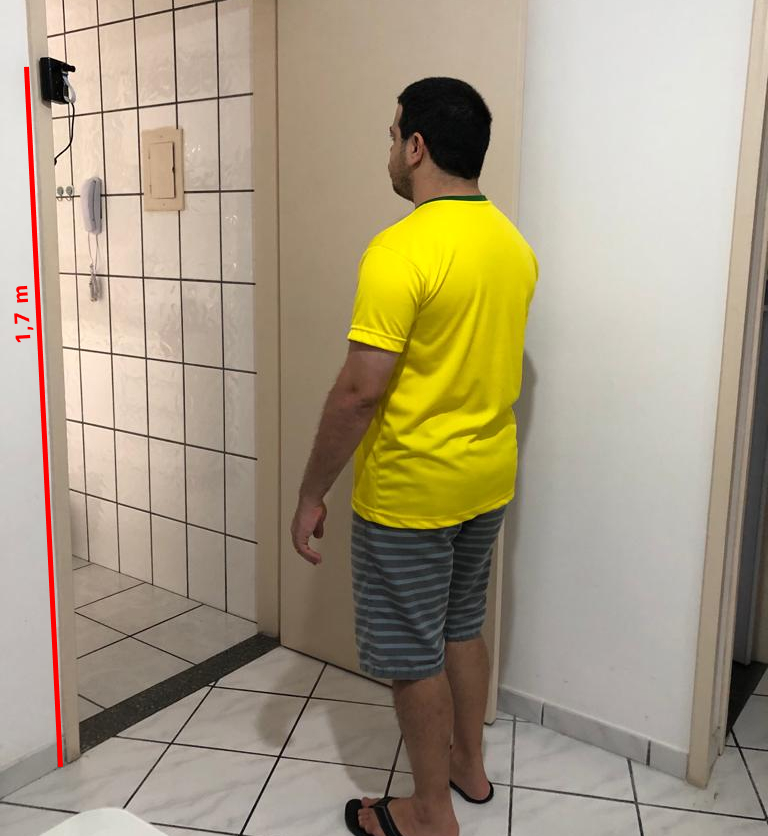
\includegraphics[width=0.65\textwidth]{Cap4_Experimentos_Realizados/Figures/cena2_posicao1_visao_externa.jpg}
    \caption*{Fonte: autor.}
    \label{fig:cena2_posicao1_visao_externa}
\end{figure}

Na figura \ref{fig:cena2_posicao1_imagem_capturada} têm-se a imagem capturada pela câmera na posição 1, na maior resolução definida para esta cena, 800x600.

\begin{figure}[H]
    \centering
    \caption[Captura da imagem na primeira posição.]{Captura da imagem na primeira posição.}
    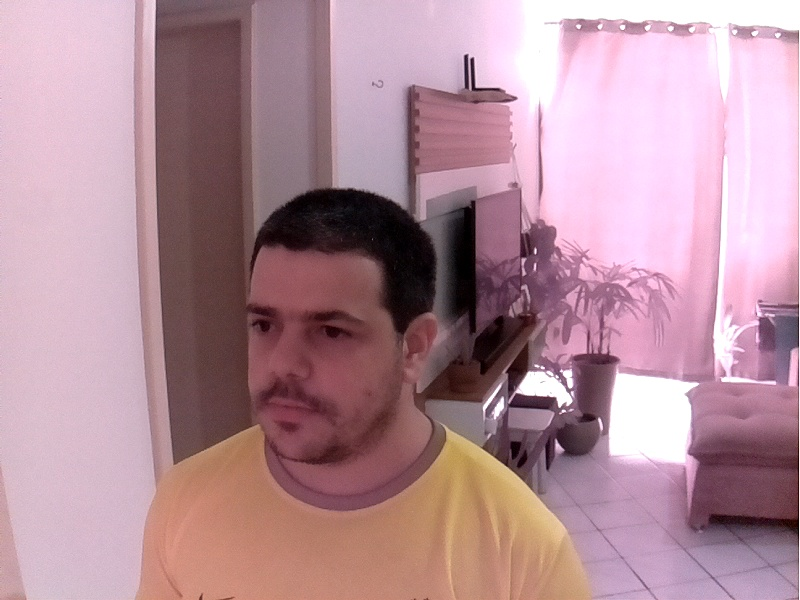
\includegraphics[width=0.65\textwidth]{Cap4_Experimentos_Realizados/Figures/cena2_posicao1_imagem_capturada.jpg}
    \caption*{Fonte: autor.}
    \label{fig:cena2_posicao1_imagem_capturada}
\end{figure}

A partir dessa primeira posição, mediu-se 1,7m distanciando-se da entrada. Essa é a posição mais distante, a partir da qual deseja-se que a face seja detectável. A figura \ref{fig:cena2_posicao2_visao_externa} demonstra esse posicionamento e na figura \ref{fig:cena2_posicao2_imagem_capturada} tem-se a imagem capturada pela câmera que também será utilizada nos testes.
\begin{figure}[H]
    \centering
    \caption[Posicionamento para captura da face na segunda posição.]{Posicionamento para captura da face na segunda posição.}
    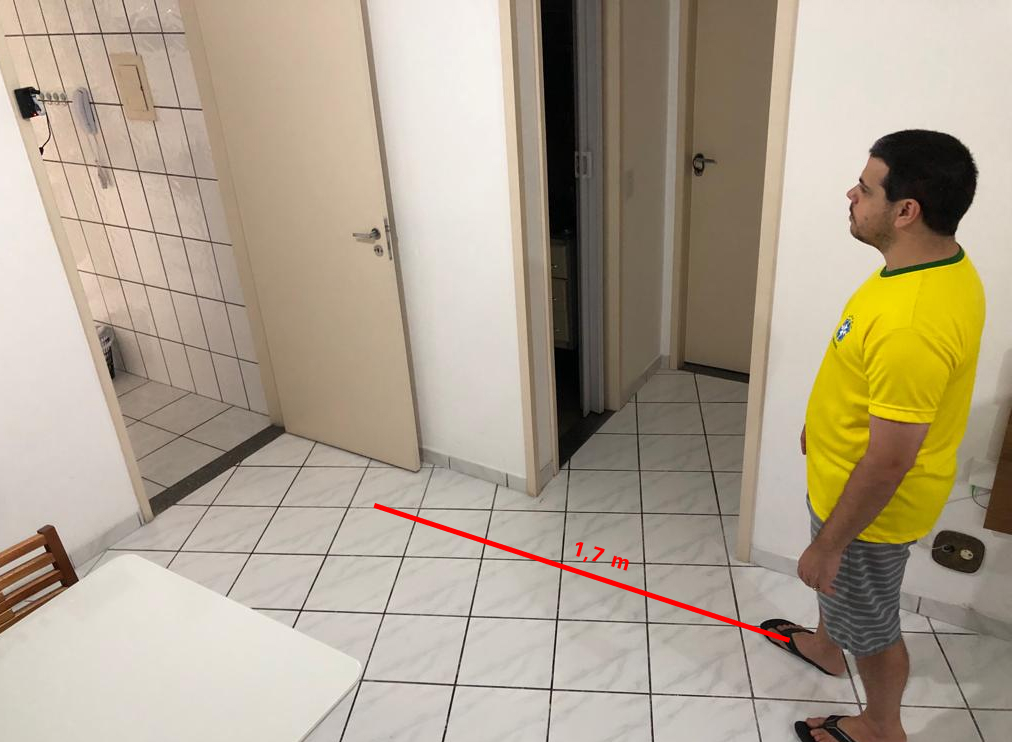
\includegraphics[width=0.65\textwidth]{Cap4_Experimentos_Realizados/Figures/cena2_posicao2_visao_externa.jpg}
    \caption*{Fonte: autor.}
    \label{fig:cena2_posicao2_visao_externa}
\end{figure}

\begin{figure}[H]
    \centering
    \caption[Captura da imagem na segunda posição.]{Captura da imagem na segunda posição.}
    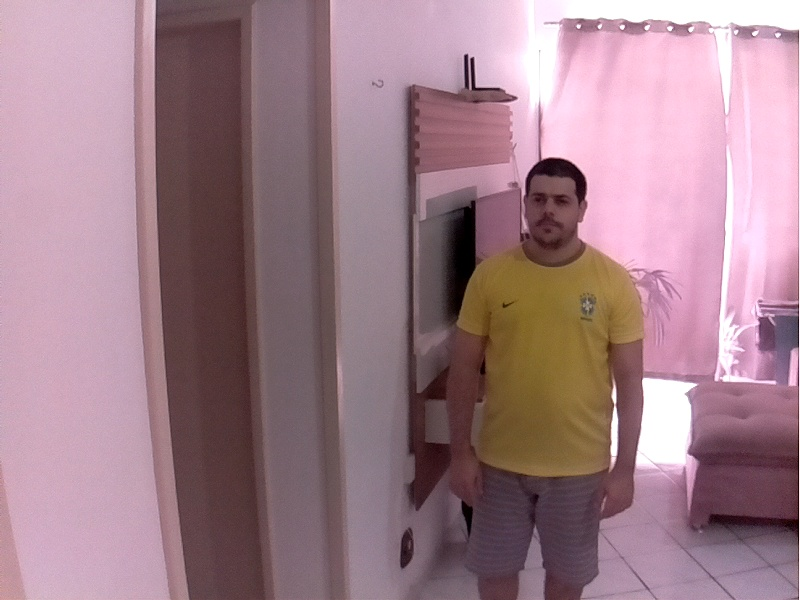
\includegraphics[width=0.65\textwidth]{Cap4_Experimentos_Realizados/Figures/cena2_posicao2_imagem_capturada.jpg}
    \caption*{Fonte: autor.}
    \label{fig:cena2_posicao2_imagem_capturada}
\end{figure}


\subsection{Otimização de parâmetros}

Foi realizada a otimização dos parâmetros para cada variação de resolução, utilizando-se as imagens capturadas nas duas posições. Utilizou-se o Raspberry Pi 4B para a definição dos parâmetros, repetindo-os nos testes com o Raspberry Pi Zero W para base de comparação.

As imagens em ambas as posições foram analisadas em conjunto mas com o objetivo de se chegar a apenas um conjunto de parâmetros 'ótimos' para obtenção das métricas. Foram considerados 'ótimos' a mesma combinação de parâmetros que atendia às duas imagens, buscando-se os limiares com o menor tempo em que as faces são detectadas e sem falsos positivos. Para facilitar a visualização desses limiares, foram definidos passos maiores de 'Scale Factor' e 'Min. Size (\%)' para se obter quantidades maiores de amostras.

Pode-se pensar, a princípio, que bastava analisar a imagem na posição 2, que é a mais distante, pois essa já seria o pior caso, já que a face teria menor resolução que a da posição 1. Porém, percebe-se claramente comparando as figuras \ref{fig:cena2_posicao1_imagem_capturada} e \ref{fig:cena2_posicao2_imagem_capturada} que quando a face está mais próxima da câmera e estando a pessoa olhando naturalmente em direção à entrada, o angulo não é muito bom, podendo criar alguma dificuldade adicional na detecção da face. Por isso a importância da análise conjunta.

Para se considerar um pior caso, foram utilizados os dados das métricas que apresentaram maiores tempos de resposta e tamanho de imagem, isso para cada resolução.

As próximas três subsubseções \ref{sssec:resolution2-1}, \ref{sssec:resolution2-2} e \ref{sssec:resolution2-3} mostram para cada resolução testada, a última iteração da matriz de resultados para a detecção em ambas as posições, com os dados entrada, a célula destacada com os parâmetros escolhidos e as imagens com a faces detectadas. Nas figuras das matrizes foram adicionadas linhas azuis (para a posição 1) e vermelhas (para aposição 2), indicando limiares que separam os grupos contínuos de resultados onde há detecção de face. Foram então selecionados os melhores resultados dentro da interseção desses grupos .

Após os parâmetros definidos no Raspberry Pi 4, os mesmos foram utilizados para obter a métricas no Raspberry Pi Zero W, sendo todos tabelados para comparação. Uma tabela resumida com esses dados é exibida no final de cada uma das próximas três subseções.

Devido ao tamanho maior das matrizes de resultados e a necessidade de visualização lado a lado, a parte da interface com os controles de parametrização não foram exibidos. Os parâmetros utilizados foram: "Min. Neighbors: 3", "Number of Samples: 6". Início e fim de escala dos demais parâmetros podem ser vistos nas matrizes.

\subsubsection{Resolução 600p} \label{sssec:resolution2-1}

A figura \ref{fig:otimizacaoCena2_600p_matrizes} apresenta lado a lado as matrizes de resultados dos testes realizados com as imagens em 600 x 800 das duas posições no Raspberry Pi 4B. Para os ranges e passos escolhidos, percebe-se que para a posição 1, com a face maior, o principal fator que delimita a região onda a face é detectada é o 'Scale Factor', com valores iguais ou menores a 1,4. Enquanto que para a posição 2, o principal delimitador para detecção da face é o 'Min. Size (\%), o que se é esperado, já que é a imagem que possui a face em tamanho menor.

As duas linha delimitadoras na cor vermelha, na matriz à direita, foram posicionadas de forma um tanto livre, mas buscando isolar regiões onde todos os resultados detectam a face. Poderia também ter sido considerada apenas uma linha horizontal entre 'Min. Size (\%) 7.0 e 8.0, por exemplo. Não mudaria muito o resultado e não teria impacto significativo na estudo.

Considerando-se o menor tempo na interseção das regiões, os parâmetros definidos foram:
\begin{itemize}
    \SingleSpacing
    \item Min. Size Face: 8.0\%
    \item Scale Factor: 1.400
    \item Min. Neighbors: 3
\end{itemize}

Os mesmos parâmetros foram utilizados para obter as métricas detalhadas nos dois dispositivos testados. Os dados obtidos são apresentados na tabela da figura \ref{fig:dadosCena2_600p} que serão usados nas comparações de resultados.

\begin{figure}[H]
    \centering
    \caption[Otimização Cena 2 - resolução 600p - matrizes. À esquerda posição 1 e à direita, posição 2]{Otimização Cena 2 - resolução 600p - matrizes. À esquerda, posição 1, e à direita, posição 2.}
    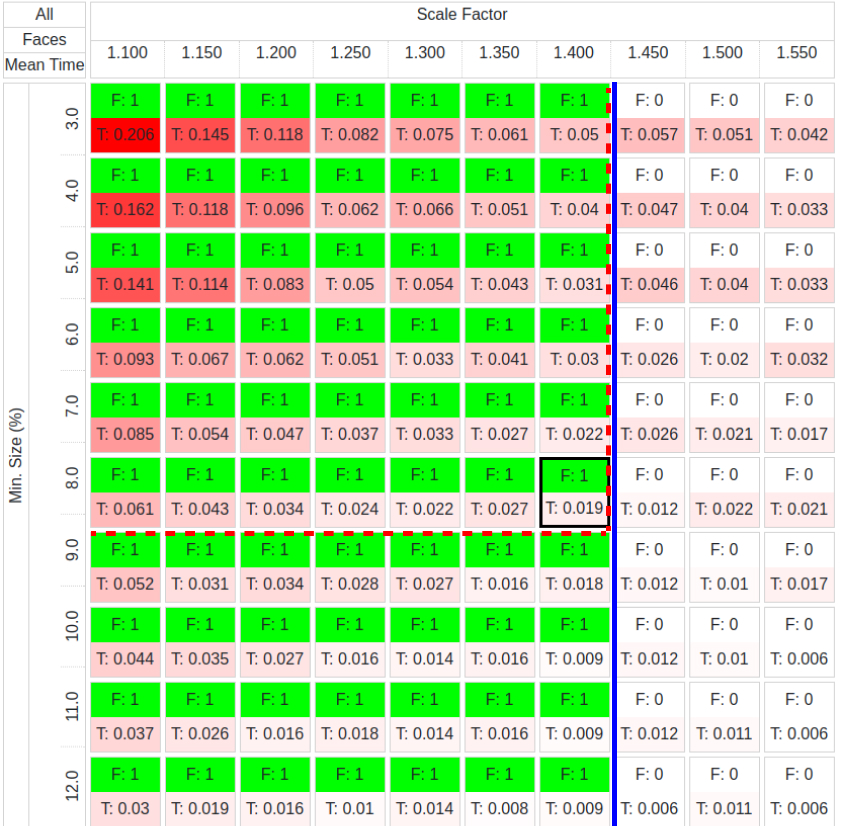
\includegraphics[width=0.49\textwidth]{Cap4_Experimentos_Realizados/Figures/cena2_800x600_pos1_matriz.jpg}
    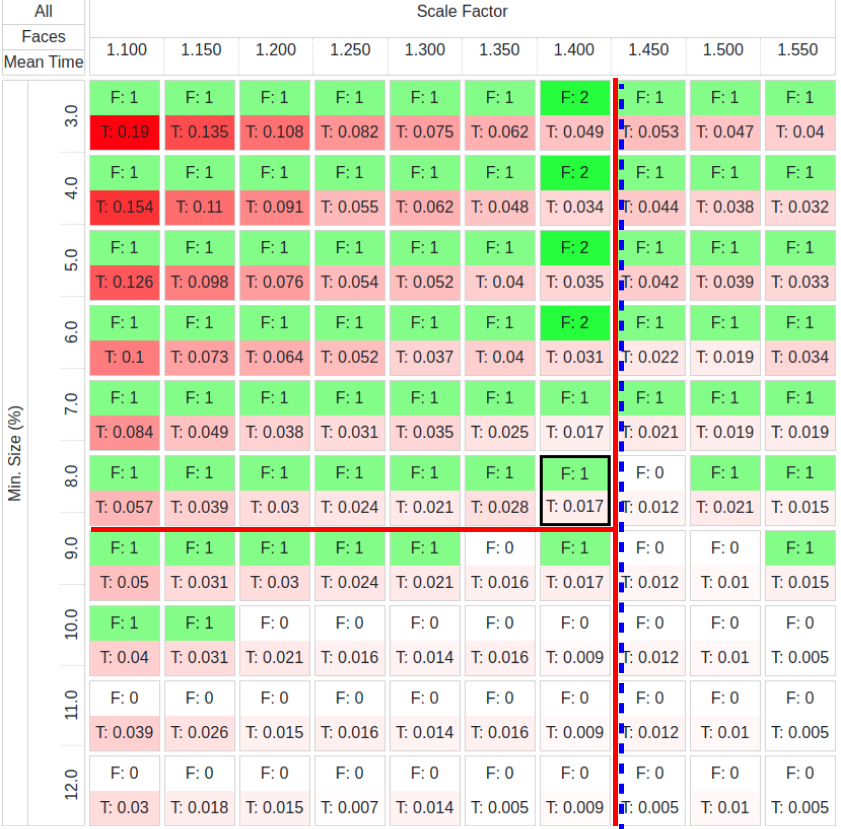
\includegraphics[width=0.49\textwidth]{Cap4_Experimentos_Realizados/Figures/cena2_800x600_pos2_matriz.jpg}
    \caption*{Fonte: autor.}
    \label{fig:otimizacaoCena2_600p_matrizes}
\end{figure}

\begin{figure}[H]
    \centering
    \caption[Otimização Cena 2 - resolução 600p - faces detectadas. À esquerda posição 1 e à direita, posição 2]{Otimização Cena 2 - resolução 600p - faces detectadas. À esquerda, posição 1, e à direita, posição 2.}
    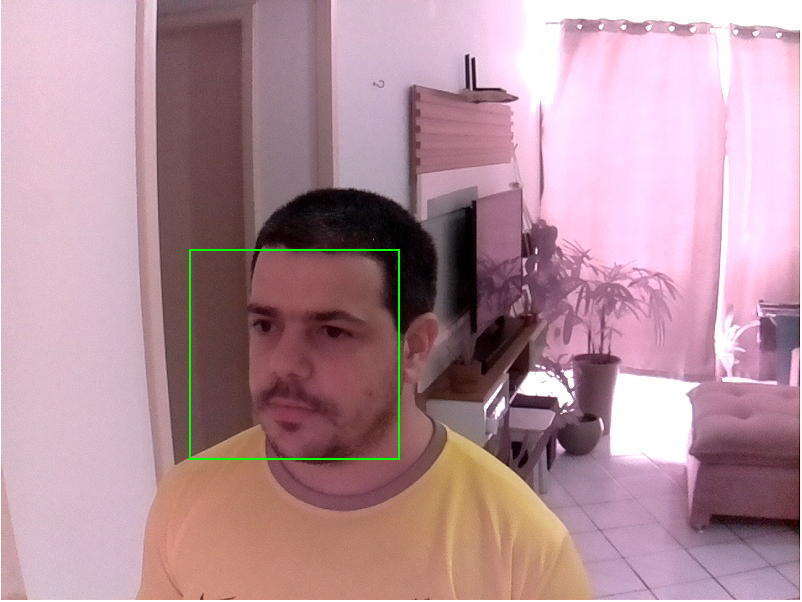
\includegraphics[width=0.49\textwidth]{Cap4_Experimentos_Realizados/Figures/cena2_800x600_pos1_face.jpg}
    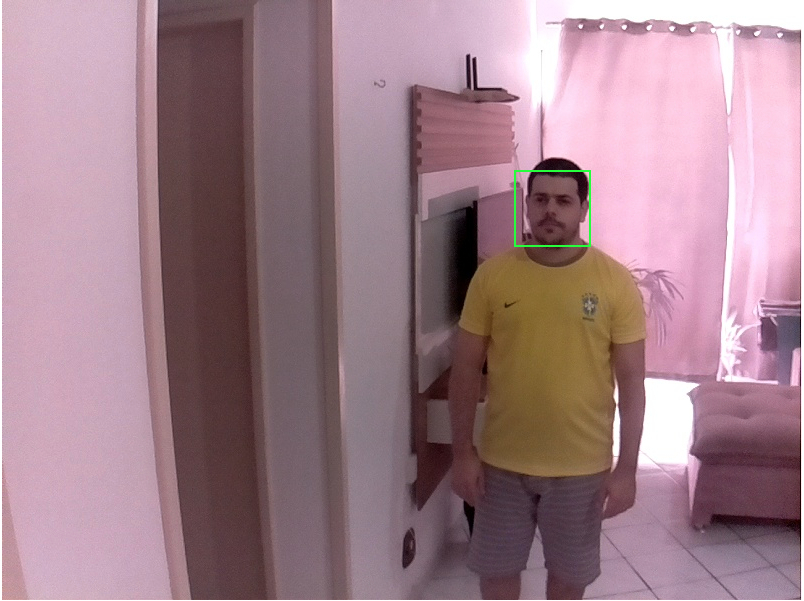
\includegraphics[width=0.49\textwidth]{Cap4_Experimentos_Realizados/Figures/cena2_800x600_pos2_face.jpg}
    \caption*{Fonte: autor.}
    \label{fig:otimizacaoCena2_600p_faces}
\end{figure}

\begin{figure}[H]
    \centering
    \caption[Tabela de Dados - resolução 600p.]{Tabela de Dados - resolução 600p.}
    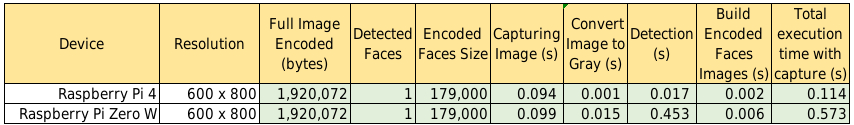
\includegraphics[width=0.90\textwidth]{Cap4_Experimentos_Realizados/Figures/cena2_dados_600p.jpg}
    \caption*{Fonte: autor.}
    \label{fig:dadosCena2_600p}
\end{figure}

\subsubsection{Resolução 480p} \label{sssec:resolution2-2}

A análise para definição dos parâmetros seguiu-se da mesma forma como já foi explicado na subsubseção anterior. Novamente a região delimitada na matriz de resultados à direita, posição 2, foi a mais restritiva.

Considerando-se o menor tempo na interseção das regiões, os parâmetros definidos foram: 
\begin{itemize}
    \SingleSpacing
    \item Min. Size Face: 8.0\%
    \item Scale Factor: 1.500
    \item Min. Neighbors: 3
\end{itemize}

A apresentação das imagens com a face detectada na figura \ref{fig:otimizacaoCena2_480p_matrizes} pode parecer repetitiva. A intenção é possibilitar uma comparação quanto à qualidade das imagens quando comparadas às da figura \ref{fig:otimizacaoCena2_600p_faces}, de maior resolução. Como não estão em seus tamanhos reais, pode ser difícil ter a percepção lendo o documento sem ampliação. Na próxima subseção as faces recortadas de cada imagem são postas lado a lado em seus tamanhos reais para possibilitar a percepção da diferença na qualidade.

\begin{figure}[H]
    \centering
    \caption[Otimização Cena 2 - resolução 480p - matrizes. À esquerda posição 1 e à direita, posição 2]{Otimização Cena 2 - resolução 480p - matrizes. À esquerda, posição 1, e à direita, posição 2.}
    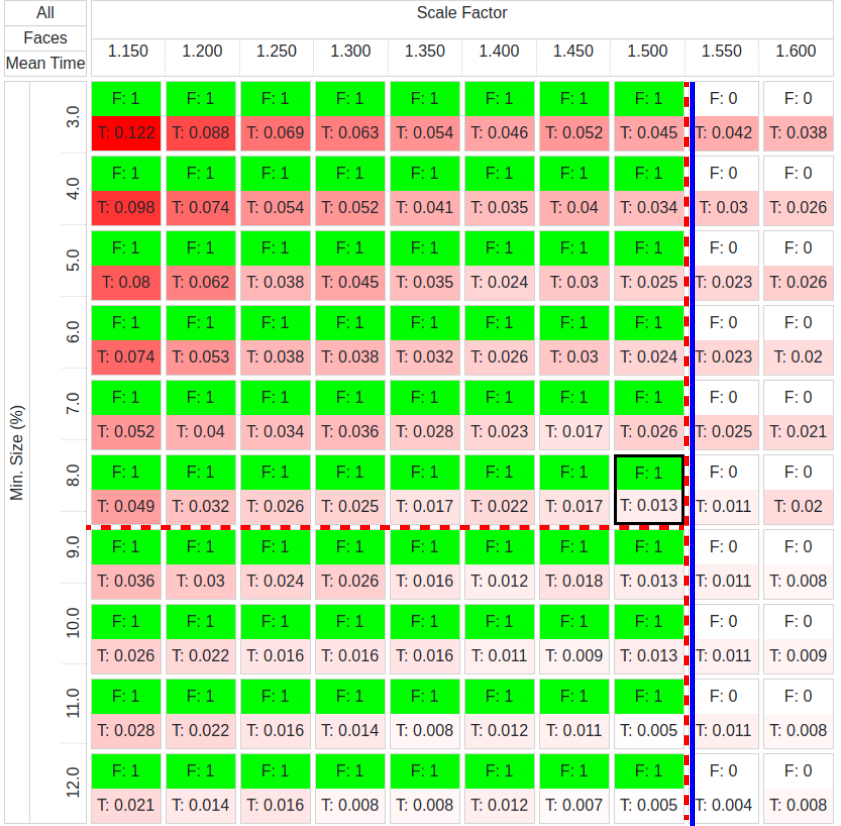
\includegraphics[width=0.49\textwidth]{Cap4_Experimentos_Realizados/Figures/cena2_640x480_pos1_matriz.jpg}
    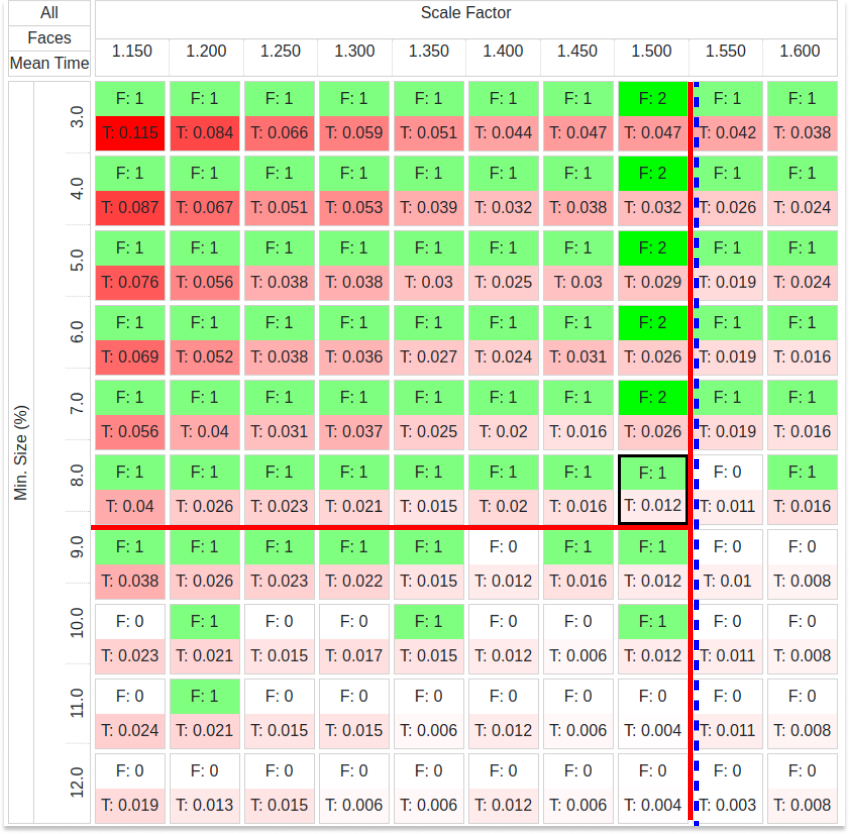
\includegraphics[width=0.49\textwidth]{Cap4_Experimentos_Realizados/Figures/cena2_640x480_pos2_matriz.jpg}
    \caption*{Fonte: autor.}
    \label{fig:otimizacaoCena2_480p_matrizes}
\end{figure}

\begin{figure}[H]
    \centering
    \caption[Otimização Cena 2 - resolução 480p - faces detectadas. À esquerda posição 1 e à direita, posição 2]{Otimização Cena 2 - resolução 480p - faces detectadas. À esquerda, posição 1, e à direita, posição 2.}
    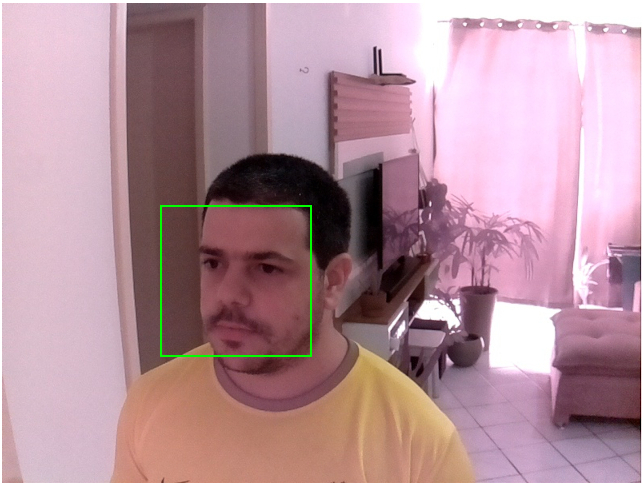
\includegraphics[width=0.49\textwidth]{Cap4_Experimentos_Realizados/Figures/cena2_640x480_pos1_face.jpg}
    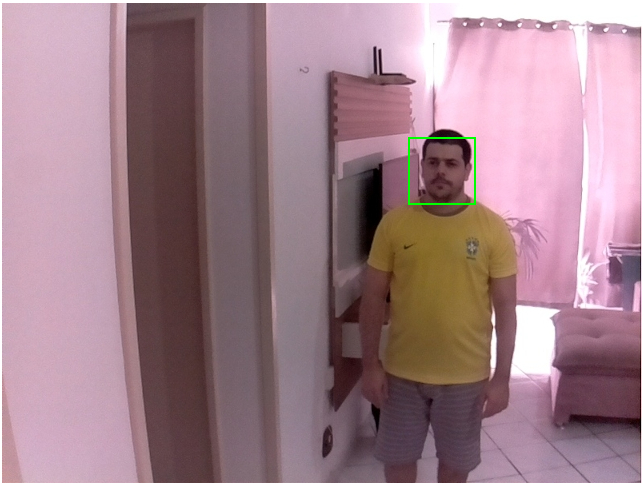
\includegraphics[width=0.49\textwidth]{Cap4_Experimentos_Realizados/Figures/cena2_640x480_pos2_face.jpg}
    \caption*{Fonte: autor.}
    \label{fig:otimizacaoCena2_480p_faces}
\end{figure}

\begin{figure}[H]
    \centering
    \caption[Tabela de Dados - resolução 480p.]{Tabela de Dados - resolução 480p.}
    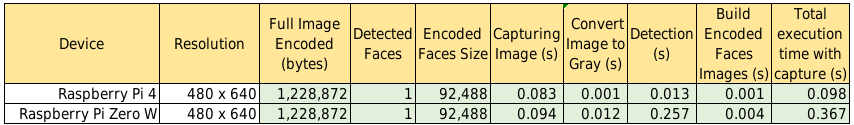
\includegraphics[width=0.90\textwidth]{Cap4_Experimentos_Realizados/Figures/cena2_dados_480p.jpg}
    \caption*{Fonte: autor.}
    \label{fig:dadosCena2_480p}
\end{figure}

\subsubsection{Resolução 240p} \label{sssec:resolution2-3}

Aa análise para definição dos parâmetros seguiu-se da mesma forma como nas subsubseções anteriores. Novamente a região delimitada na matriz de resultados à direita, posição 2, foi a mais restritiva.

Considerando-se o menor tempo na interseção das regiões, os parâmetros definidos foram: 
\begin{itemize}
    \SingleSpacing
    \item Min. Size Face: 7.0\%
    \item Scale Factor: 1.250
    \item Min. Neighbors: 3
\end{itemize}

\begin{figure}[H]
    \centering
    \caption[Otimização Cena 2 - resolução 240p - matrizes. À esquerda posição 1 e à direita, posição 2]{Otimização Cena 2 - resolução 240p - matrizes. À esquerda, posição 1, e à direita, posição 2.}
    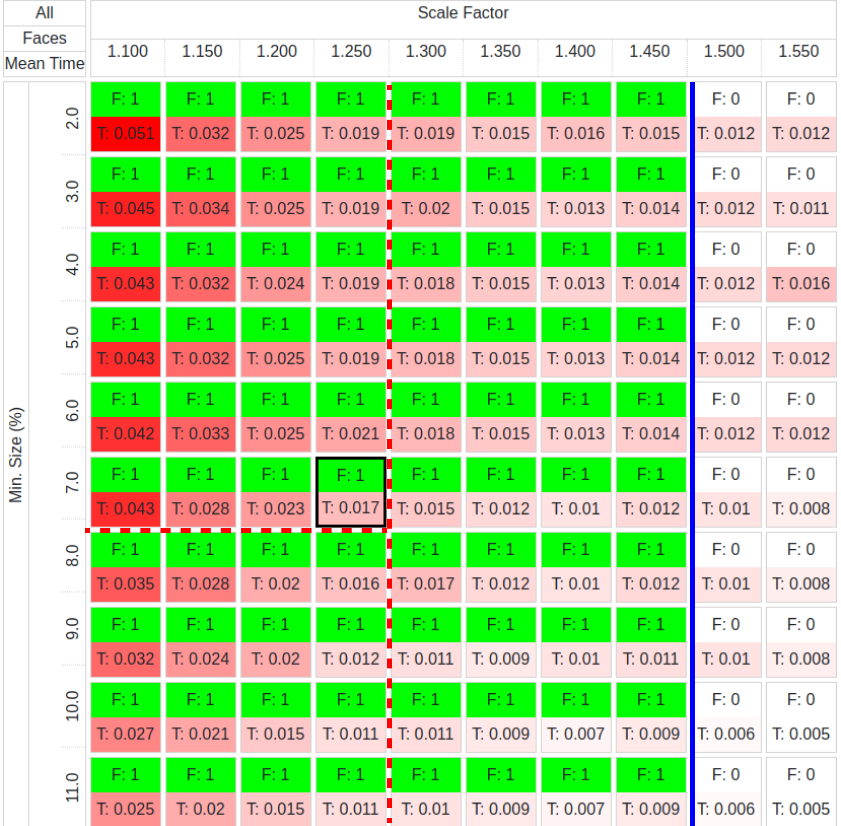
\includegraphics[width=0.49\textwidth]{Cap4_Experimentos_Realizados/Figures/cena2_320x240_pos1_matriz.jpg}
    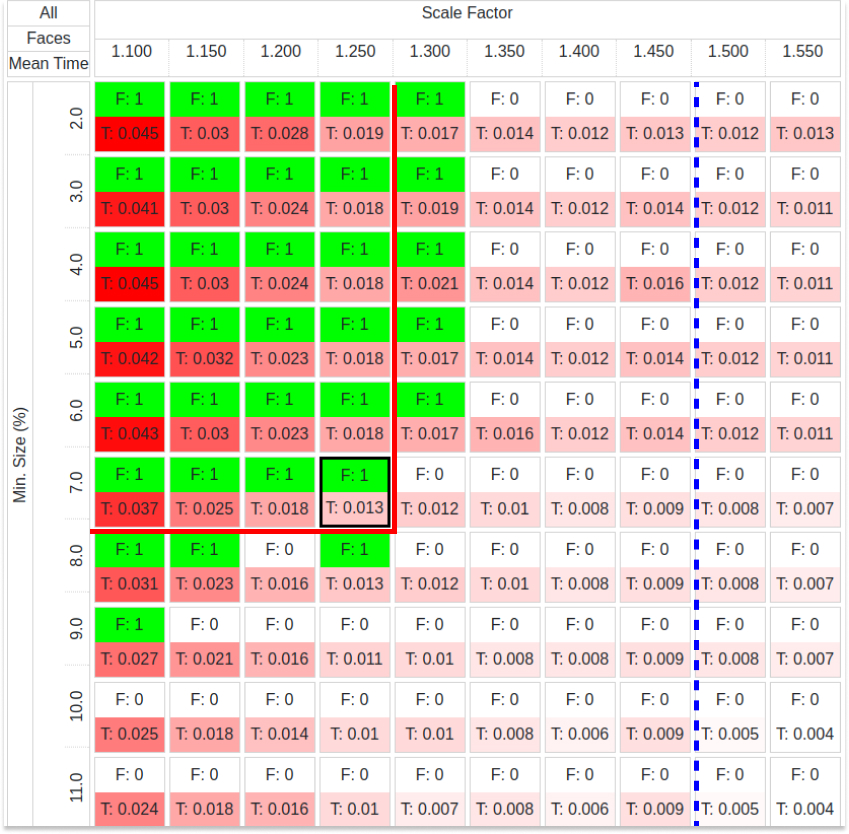
\includegraphics[width=0.49\textwidth]{Cap4_Experimentos_Realizados/Figures/cena2_320x240_pos2_matriz.jpg}
    \caption*{Fonte: autor.}
    \label{fig:otimizacaoCena2_240p_matrizes}
\end{figure}

Nessa resolução, já se consegue perceber mais claramente a diferença da qualidade das imagens apresentadas na figura \ref{fig:otimizacaoCena2_240p_faces} se comparadas às imagens das figuras \ref{fig:otimizacaoCena2_480p_faces} e \ref{fig:otimizacaoCena2_600p_faces}, com resoluções maiores.

\begin{figure}[H]
    \centering
    \caption[Otimização Cena 2 - resolução 240p - faces detectadas. À esquerda posição 1 e à direita, posição 2]{Otimização Cena 2 - resolução 240p - faces detectadas. À esquerda, posição 1, e à direita, posição 2.}
    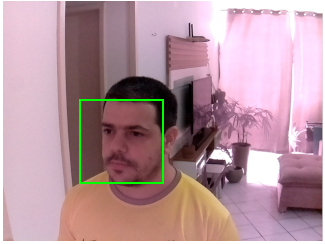
\includegraphics[width=0.49\textwidth]{Cap4_Experimentos_Realizados/Figures/cena2_320x240_pos1_face.jpg}
    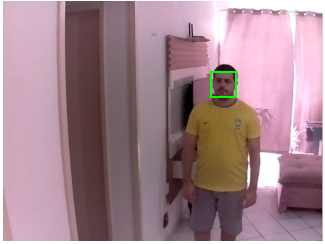
\includegraphics[width=0.49\textwidth]{Cap4_Experimentos_Realizados/Figures/cena2_320x240_pos2_face.jpg}
    \caption*{Fonte: autor.}
    \label{fig:otimizacaoCena2_240p_faces}
\end{figure}

\begin{figure}[H]
    \centering
    \caption[Tabela de Dados - resolução 240p.]{Tabela de Dados - resolução 240p.}
    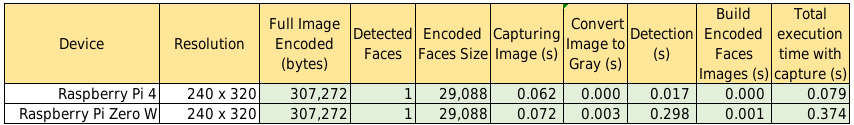
\includegraphics[width=0.90\textwidth]{Cap4_Experimentos_Realizados/Figures/cena2_dados_240p.jpg}
    \caption*{Fonte: autor.}
    \label{fig:dadosCena2_240p}
\end{figure}

\subsection{Análise dos resultados}

Nesta cena, são dois os fatores que influenciam no resultado das detecções, que são a resolução da imagem e o dispositivo rodando o algoritmo de detecção, sobre os quais serão feitas as comparações e análises a seguir.

Os dados das métricas em todas as resoluções foram obtidos a partir da imagem na posição 1, pois apresentou maiores tempos de resposta e maiores tamanhos de imagem da face recortada em relação à posição 2, sendo assim o pior caso.

\subsubsection{Efeitos da variação por resolução de imagem e considerações sobre os dispositivos testados}

O gráfico da figura \ref{fig:cena2_graficos_variacao_resolucao} compara o tempo de resposta entre os dois dispositivos testados, linhas azuis claro e escuro, e nas diferentes resoluções, distribuídas no eixo x. Também foi representado no gráfico o tempo máximo de resposta estabelecido na cena, 0,3 segundo, linha tracejada amarela. 

\begin{figure}[h]
    \centering
    \caption[Tempos de execução por Variação de resolução.]{Tempos de execução por Variação de resolução.}
    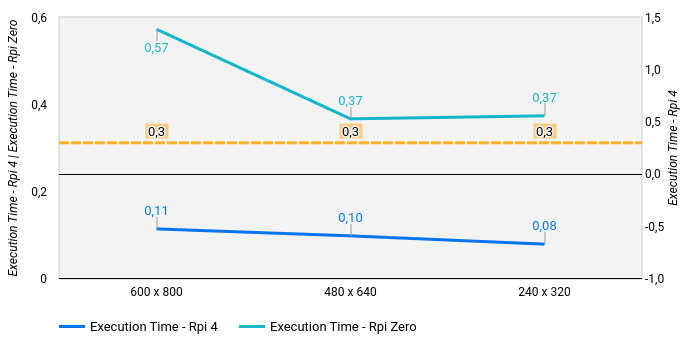
\includegraphics[width=0.7\textwidth]{Cap4_Experimentos_Realizados/Figures/cena2_graficos_variacao_resolucao.jpg}
    \caption*{Fonte: autor.}
    \label{fig:cena2_graficos_variacao_resolucao}
\end{figure}

Como pode ser observado, os tempos de resposta do Raspberry Pi 4B ficaram bem abaixo do do tempo máximo definido para esta cena, chegando a no máximo 0,11 segundo (63\% de margem), na resolução de 600 x 800, e reduzindo não muito expressivamente à medida que se reduz a resolução da imagem. Com isso, pode-se concluir que o Raspberry Pi 4B é capaz de realizar a detecção de faces únicas em tempo suficientemente pequeno para atender aos requisitos da cena nas três resoluções testadas. Isso significa que, considerando-se o cenário estabelecido e o ciclo de detecção rodando a cada 0,3s, o dispositivo é capaz de obter a imagem e realizar a detecção da face (se a posição for favorável) de uma mesma pessoa pelo menos três vezes, considerando-se essa pessoa caminhando rapidamente em direção à entrada do ambiente (um pior caso), conforme demonstrado na subsubseção \ref{sssec:memoria_calculo}.

Quanto à margem de pelo menos 63\% no tempo de resposta do Raspberry Pi 4B, pode-se pensar em aproveitá-la de pelo menos duas formas. Uma delas seria considerar um período menor no ciclo de detecção. Se o ciclo de detecção rodar conforme o tempo de resposta do dispositivo e não a cada 0,3s, a quantidade de frames capturados e analisados de uma mesma pessoa pode chegar a aproximadamente 10. Outra possibilidade seria a sobra de tempo de processamento para realizar outros tratamentos ou análises na imagem, como por exemplo o reconhecimento da face detectada. Realizar o reconhecimento de face na borda poderia gerar consideráveis ganhos em aplicações distribuídas, assunto que poderia ser objeto de um estudo futuro.

Uma questão interessante a se observar é quanto à parcela de cada etapa de processamento no tempo total de resposta. A figura \ref{fig:cena2_parcelas_etapas_resolucao_rapi4} mostra o gráfico em barras empilhadas mostrando a contribuição no tempo de execução de cada etapa, no Raspberry Pi 4B, por cada resolução. Como pode ser observado, as etapas de converter a imagem para escala de cinza (barra amarela) e o encodamento das faces recortadas (barra laranja) têm tempos de execução tão pequenos, que foram aproximados a 0 na precisão de 2 casas decimais, podendo ser considerados então insignificantes nesse caso.

Quando se os tempos mais significantes observa-se que o tempo de execução de captura da imagem (em azul) é consideravelmente maior que o tempo de execução da própria detecção de faces em si, isso para todas as resoluções. Verifica-se também que a variação no tempo total de execução, dá-se por influência majoritária do tempo de captura dos frames que, logicamente, são menores conforme se reduz a resolução da imagem. 

\begin{figure}[h]
    \centering
    \caption[Parcela de cada etapa no tempo de execução no Raspberry Pi 4, por resolução.]{Parcela de cada etapa no tempo de execução no Raspberry Pi 4, por resolução.}
    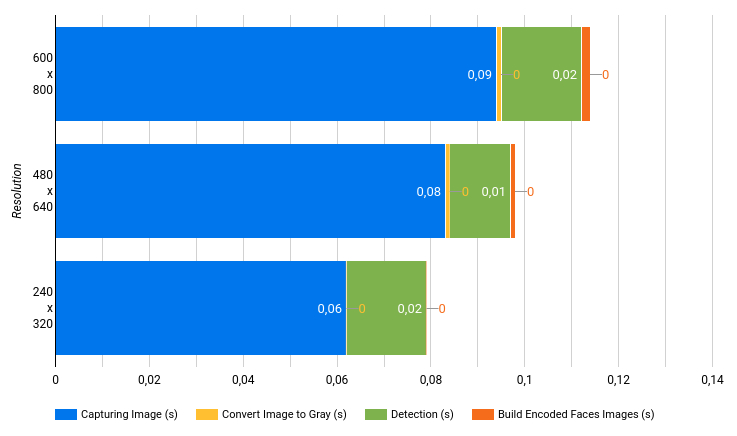
\includegraphics[width=0.95\textwidth]{Cap4_Experimentos_Realizados/Figures/cena2_parcelas_etapas_resolucao_rapi4.jpg}
    \caption*{Fonte: autor.}
    \label{fig:cena2_parcelas_etapas_resolucao_rapi4}
\end{figure}

Importante ressaltar também que existe ainda o potencial de se reduzir ainda mais o tempo de resposta total implementando-se estratégia de processamento assíncrono entre a etapa de captura de frames e as demais, o que não foi feito para este estudo.

Com relação a qual das resoluções adotar, ainda analisando-se os resultados obtidos com o Raspberry Pi 4B, poderia-se dizer a menor resolução (240 x 320) seria a mais adequada em se considerando apenas tempo de resposta. A utilização da menor resolução também irá proporciona a vantagem de utilizar menor largura de banda para trafegar os dados das imagem na rede e também ocuparia menor espaço de armazenamento (se for o caso).

Porém, se a qualidade das imagens das faces for um fator importante para posteriores tratamentos das imagens dentro da aplicação, a escolha de se utilizar as resoluções maiores pode fazer grande diferença. Para demonstrar isso, as figuras \ref{fig:cena2_comparativo_qualidade_faces_tamanho_real} e \ref{fig:cena2_comparativo_qualidade_faces_tamanho_proporcional}, fazem comparativos entre as faces recortadas nas duas posições e nas diferentes resoluções. Na figura \ref{fig:cena2_comparativo_qualidade_faces_tamanho_real}, as imagens estão apresentadas nas proporções reais entre si, considerando-se seu tamanho real, em pixels. Na figura \ref{fig:cena2_comparativo_qualidade_faces_tamanho_proporcional}, as faces de resoluções menores foram alargadas de forma que todas as faces ficassem aproximadamente do mesmo tamanhos. Assim, é possível perceber com clareza a diferença na qualidade da imagens. Na face menor recortada da resolução 240 x 320 é evidente a perda de definição nos detalhes da face, algo que poderia fazer toda a diferença na qualidade do resultado de um reconhecimento de face, por exemplo.

\begin{figure}[h]
    \centering
    \caption[Comparativo de faces recortadas de diferentes resoluções, em tamanho real.]{Comparativo de faces recortadas de diferentes resoluções, em tamanho real.}
    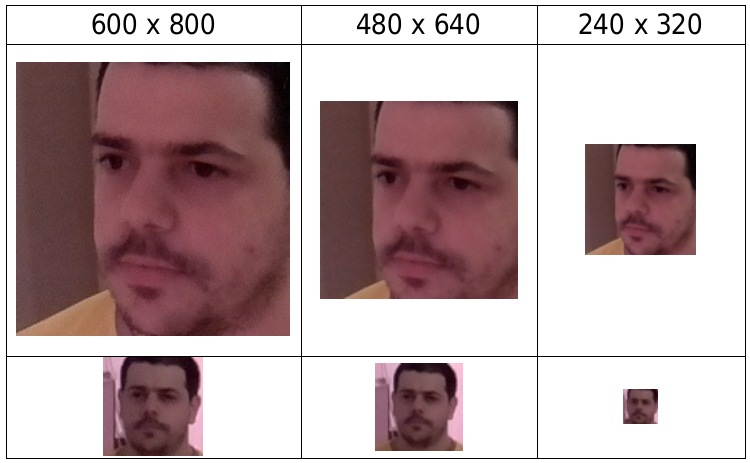
\includegraphics[width=0.8\textwidth]{Cap4_Experimentos_Realizados/Figures/cena2_comparativo_qualidade_faces_recortadas_tamanho_real.jpg}
    \caption*{Fonte: autor.}
    \label{fig:cena2_comparativo_qualidade_faces_tamanho_real}
\end{figure}

\begin{figure}[h]
    \centering
    \caption[Comparativo de faces recortadas de diferentes resoluções, em tamanhos ajustados.]{Comparativo de faces recortadas de diferentes resoluções, em tamanhos ajustados.}
    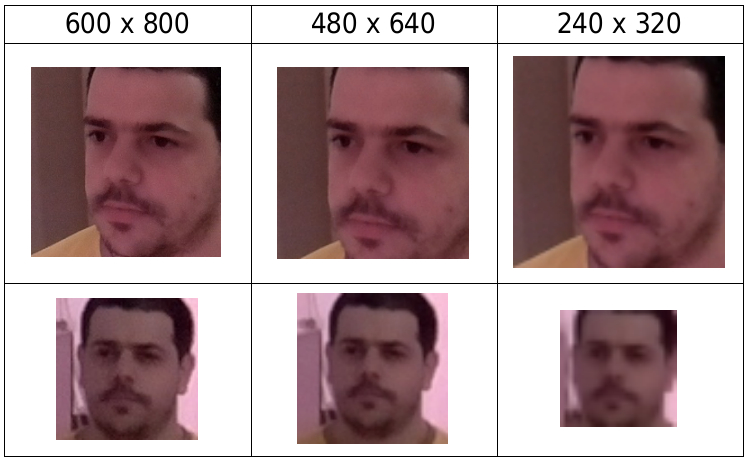
\includegraphics[width=0.8\textwidth]{Cap4_Experimentos_Realizados/Figures/cena2_comparativo_qualidade_faces_recortadas_tamanho_proporcional.jpg}
    \caption*{Fonte: autor.}
    \label{fig:cena2_comparativo_qualidade_faces_tamanho_proporcional}
\end{figure}

Quanto aos resultados do Raspberry Pi Zero W, observa-se na figura \label{fig:cena2_graficos_variacao_resolucao} que na maior resolução, o tempo de resposta foi relativamente alto, 0,57s, quase o dobro do limite máximo definido. Ao se utilizar resoluções menores, 480 x 640 e 240 x 320, o tempo de resposta reduziu consideravelmente, chegando a 0,37s em ambos os casos, apenas 0,07s acima do limite estabelecido para a cena. Por conta disso poderia-se considerar que o uso desse dispositivo não seria muito adequado para esse tipo de cena, porém, pode-se considerar algumas possibilidades de melhoria. Por exemplo, a otimização de todo o processo utilizando-se técnicas de processamento assíncrono ou o teste de resoluções ainda menores têm o potencial de apresentar reduções consideráveis no tempo de resposta. Ou então a aplicação em cenários com critérios um pouco diferentes podem tornar esses tempos de respostas mais aceitáveis, como por exemplo em casos em que seja considerado um tempo maior de exposição das faces em frente à câmera.

Em termos apenas de performance, a utilização do Raspberry Pi 4B é mais recomendada, considerando-se que o tempo de resposta chega a ser em torno de 78\% menor do que o observado no Raspberry Pi Zero W. Porém, há outros fatores que podem ser decisivos na escolha do dispositivo a ser utilizado em um projeto, como o valor e o tamanho. O Raspberry Pi Zero W custa em torno de 73\% menos que o Raspberry Pi 4B \footnote{Conforme preços encontrandos em visita à loja online com endereço www.robocore.net, no dia 30/11/2022. Como não havia disponível para venda o modelo exato do Raspberry Pi Zero W, foi considerado o valor do Raspberry Pi Zer 2 W, que possui configurações de hardware semelhantes.} e possui área em torno de 59\% menor . O desempenho do Raspberry Pi Zero W não atendeu totalmente aos requisitos definidos para este cenário específico, porém se mostrou muito promissor. Caso fatores de custo e/ou dimensões sejam relevantes para o projeto, vale a pena considerá-lo como opção.

\subsubsection{Considerações sobre utilização de banda}

Considerando-se uma possível aplicação com arquitetura distribuída, a figura \ref{fig:cena2_comparativo_utilizacao_banda} mostra um comparativo de como seria a utilização de banda em dois possíveis casos, transmissão da imagem completa capturada pelo dispositivo da borda para outro dispositivo realizar a detecção, e transmissão apenas as imagens das
faces já detectadas e recortadas pelo dispositivo na borda. Para o cálculo de utilização de banda, considerou-se intervalo entre as detecções de 0,3 segundo, conforme tempo
máximo definido como requisito para esta cena.

São apresentados os resultados por resolução de imagem, eixo x. Nas barras de cor vermelha têm-se a largura de banda que seria utilizada trafegando-se a imagem completa e nas barras de cor verde a largura de banda considerando-se o tráfego apenas do recorte das faces detectadas, ambas seguindo a escala à esquerda do eixo y e expressas em MBps. Na série em formato de linha azul têm-se a diferença percentual em relação ao tamanho da imagem completa, seguindo a escala à direita do eixo y.

\begin{figure}[h]
    \centering
    \caption[Comparativo de utilização de banda.]{Comparativo de utilização de banda.}
    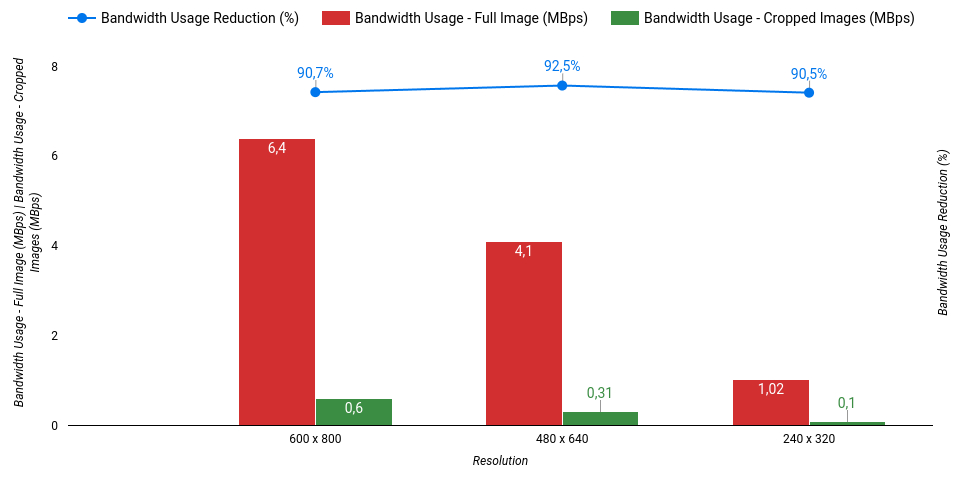
\includegraphics[width=0.95\textwidth]{Cap4_Experimentos_Realizados/Figures/cena2_comparativo_utilizacao_banda.jpg}
    \caption*{Fonte: autor.}
    \label{fig:cena2_comparativo_utilizacao_banda}
\end{figure}

Como pode-se observar, a redução na utilização de banda é bastante expressivo quando se processa a detecção de faces na borda, variando em torno de 90\% e 93\% entre as diferentes resoluções. Importante ressaltar que esses dados foram obtidos a partir da imagem da posição 1, quando o tamanho da face é maior. Ou seja, na média, esse ganho na redução tende a ser um pouco maior já que haverá frames capturados com faces menores, chegando a até 100\% quando não houver face presente.

Reforçando-se que as unidades no gráfico estão em MBps e não em Mbps e considerando-se as imagens trafegando em uma rede de 100 MBps, transmitir a imagem completa na resolução 600 x 800 utilizaria em média 51\% de toda a banda, para apenas esse dispositivo, enquanto que transmitir apenas as imagens das faces recortadas utilizaria em torno de 5\% da banda da rede, em média.

Novamente, em uma aplicação real, é razoável considerar que podem haver dezenas de dispositivos realizando monitoramento e tendo de enviar imagens e dados a algum outro dispositivo centralizador. A tabela apresentada na figura \ref{fig:cena2_tabela_qtde_disp_resolucao} apresenta um comparativo de quanto seria a utilização média de banda para diferentes quantidades de dispositivos transmitindo as imagens das faces detectadas simultaneamente em uma mesma rede. São apresentados os valores para cada resolução testada.

\begin{figure}[h]
    \centering
    \caption[Utilização de banda em Mbps por quantidade de dispositivos e resolução.]{Utilização de banda em Mbps por quantidade de dispositivos e resolução.}
    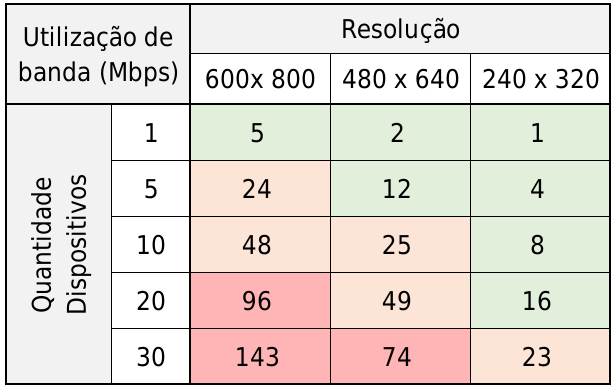
\includegraphics[width=0.40\textwidth]{Cap4_Experimentos_Realizados/Figures/cena2_tabela_qtde_disp_resolucao.jpg}
    \caption*{Fonte: autor.}
    \label{fig:cena2_tabela_qtde_disp_resolucao}
\end{figure}

Primeiramente, os dados da tabela mostram que, com a detecção de faces sendo processada pelo dispositivo de borda, a implementação de vários desses dispositivos funcionando simultaneamente em uma mesma rede se torna viável, graças à transmissão apenas das partes úteis das imagens. Outra questão que se observa é o quão importante se torna a escolha da resolução da imagem nesses casos. Dependendo da quantidade de dispositivos, a utilização da resolução 600 x 800 se tornaria inviável em uma rede de 100 Mbps, como é o caso de 20 dispositivos por exemplo, que ocuparia até 96\% da banda disponível. Porém, para essa mesma quantidade na resolução de 240 x 320, a utilização de banda já cairia drasticamente para um máximo de 16\%, claro que a custo da qualidade da imagem.